% Sema: Content-Addressed Semantics for Multi-Agent Coordination

\documentclass[11pt,a4paper]{article}
\usepackage[utf8]{inputenc}
\usepackage{xcolor}
\usepackage{listings}
\usepackage{booktabs}
\usepackage{multirow}
\usepackage{float}      % For [H] placement
\usepackage{graphicx}
\usepackage{amsmath}
\usepackage{amsfonts}
\usepackage{amssymb}
\usepackage{amsthm}
\usepackage{emergentwisdom-preprint}
\usepackage{microtype}  % Improved typography
\usepackage{tikz}       % For diagrams
\usepackage{needspace}  % Keep generated taxonomy headings with their first item
\usepackage{placeins}   % Keep explanatory text behind its associated floats
\usepackage{hyperref}   % Load last so float and section anchors use their final definitions
\hypersetup{
  hidelinks,
  pdftitle={Sema: When the Hash Is the Word},
  pdfauthor={Henrik Westerberg},
  pdfsubject={Content-addressed semantics for verifiable multi-agent coordination},
  pdfkeywords={content-addressed semantics, multi-agent systems, verifiable references, semantic coordination, Merkle commitments, agent vocabularies, pattern cards}
}
\usetikzlibrary{positioning, shapes, arrows.meta, calc, shadows}

\newtheorem{proposition}{Proposition}

% Import auto-generated statistics
% Auto-generated stats from calculate_graph_stats.py
\newcommand{\semaPatternCount}{453}
\newcommand{\semaTotalNodes}{2,895}
\newcommand{\semaTotalEdges}{4,072}
\newcommand{\semaAvgEdges}{9.0}
\newcommand{\semaInvariantCount}{788}
\newcommand{\semaPrinciplesCount}{552}
\newcommand{\semaPatternsWithInvariants}{366}
\newcommand{\semaInvariantPct}{80\%}
\newcommand{\semaPatternsWithPre}{194}
\newcommand{\semaPrePct}{42\%}
\newcommand{\semaPatternsWithPost}{183}
\newcommand{\semaPostPct}{40\%}
\newcommand{\semaPatternsWithIO}{70}
\newcommand{\semaIOPct}{15\%}
\newcommand{\semaPatternsWithParams}{98}
\newcommand{\semaParamPct}{21\%}
\newcommand{\semaPatternsWithCompose}{78}
\newcommand{\semaComposePct}{17\%}
\newcommand{\semaTotalParams}{211}


% Custom colors
\definecolor{semablue}{RGB}{0, 70, 140}
\definecolor{semagreen}{RGB}{0, 100, 60}
\definecolor{semared}{RGB}{140, 20, 20}
\definecolor{jsonkey}{RGB}{0, 50, 150}
\definecolor{graybg}{gray}{0.96}

% Code listing style (enhanced for JSON)
\lstset{
  basicstyle=\ttfamily\small,
  breaklines=true,
  frame=lines,
  backgroundcolor=\color{graybg},
  keywordstyle=\color{jsonkey}\bfseries,
  commentstyle=\color{green!60!black},
  stringstyle=\color{orange!80!black},
  numbers=left,
  numberstyle=\scriptsize\color{gray},
  numbersep=8pt
}

% Custom commands for Sema patterns
\newcommand{\sema}[2]{\texttt{#1}\allowbreak\texttt{\##2}}
\newcommand{\apl}[1]{\texttt{#1}}
\newcommand{\hash}{\mathcal{H}}
\newcommand{\vocab}{\mathcal{V}}

\title{Sema: When the Hash Is the Word}
\renewcommand{\shorttitle}{Sema: When the Hash Is the Word}
\author{Henrik Westerberg\\Emergent Wisdom\\\texttt{henrik.westerberg@emergentwisdom.org}}
\ewrevisedtoday{April 7, 2026}

\begin{document}

\maketitle

\begin{abstract}
Autonomous agents often reason and coordinate through labels that do not reveal which external information they denote. We present Sema, a content-addressed reference system for reasoning and communication that creates \emph{verifiable words}: participants encode and hash information under an agreed representation, then reuse the content address as a term, optionally with a human-readable handle. Sema can use any representation if participants agree on how content is encoded, hashed, resolved, and decoded. This paper develops one concrete realization based on canonicalized JSON-compatible objects, field-level Merkle commitments, explicit identity rules, and content-addressed references. Full-reference verification establishes identity of the resolved hashed content, while semantic equivalence, correctness, and compliance remain separate questions.

As a worked application of the Sema primitive, we introduce Pattern Cards, a concrete schema for deliberate, System~2-style reasoning. They make often-skipped reasoning moves explicit through contracts for mechanisms, conditions, invariants, typed dependencies, and failure modes. Within one agent, resolving a card can make a reusable reasoning procedure explicit. Across agents, the same content-addressed definitions support coordination: agents can verify that they resolved the same definitions; in strict mode, an enforced handshake halts on mismatch.

A bootstrap library of \semaPatternCount~cards demonstrates the design. Its contract fields averaged \semaLibCompRatio~times the tokens of short wire references---a transmission-compression result, not an inference-token saving, because definitions were hydrated before use. Illustrative agent demonstrations examine coordination behavior. The same primitive could support a Living Taxonomy of Thought; its utility, evolution, and governance remain open questions.
\end{abstract}

\keywords{Content-Addressed Semantics, Multi-Agent Systems, Verifiable References, Semantic Coordination, Merkle Commitments, Agent Vocabularies, Pattern Cards}

%==============================================================================
\section{Introduction}
%==============================================================================

We are entering the era of the \emph{Agent Web}, where autonomous AI systems negotiate resources, execute code, delegate tasks, and make consequential decisions across organizational boundaries. Yet an ordinary label in an agent message does not reveal which external definition its sender intends. Without an explicit resolution and verification step, apparently shared terms can conceal different specifications. Five problems motivate such a step:

\begin{description}
\item[The Paraphrase Problem.] Agent~A may need to reproduce a lengthy behavioral specification for Agent~B, and each paraphrase risks drifting from the last. A reusable reference could carry the identity of that specification more compactly.

\item[The Identity Problem.] When two agents use the phrase ``coordinate safely,'' the label alone does not establish that they refer to the same external definition. Silent divergence can compound through agent chains where identical labels hide different specifications.

\item[The Hallucination Problem.] Large Language Models fabricate references and citations~\cite{gibney2025hallucination}, motivating a ``fail-closed'' architecture that checks references against their resolved content. A fabricated or mismatching pointer can then be rejected; whether verified content is relevant or correct remains a separate question.

\item[The Trust Problem.] RDF and OWL provide shared representation frameworks, but do not by themselves verify that low-trust peers resolved the same external definition.

\item[The Granularity Problem.] A generic report that ``the coordination failed'' leaves the cause open, whereas ``the Lock Invariant in \sema{StateLock}{c9c2} was violated at $t=3.2$s'' identifies the clause being assessed. A vocabulary of named contracts gives agents and their evaluators a more precise diagnostic language. Detecting the violation still requires observation and checking.
\end{description}

Ordinary communication leaves many reusable procedures unnamed or defined anew at each use. A resolvable agent vocabulary makes additional names practical: detailed definitions can be expanded on demand, allowing recurring procedures to become precise, composable terms without requiring every participant to memorize the whole library.

Sema\footnote{The name ``Sema'' (Greek \textit{s\={e}ma}, ``sign'') was chosen in December 2025. An unrelated system also named SEMA~\cite{feng2026sema}, addressing multi-turn jailbreak attacks on LLMs, appeared at ICLR 2026. The two systems share only the acronym and operate at different layers (definition-identity verification vs.\ attack methodology).} is a communication primitive: hash information under an agreed representation and carry the resulting content address directly in communication. Its agent-coordination application assumes a low-trust environment where agents may hallucinate, drift, or actively deceive. This paper develops a JSON/Merkle realization for behavioral definitions called Pattern Cards.

Content-addressing definitions has clear precedents in Hawke's Semantic Definition Hash (SDH)~\cite{sdh2002}, Trusty URIs~\cite{kuhn2014trusty}, and systems such as Git, IPFS~\cite{benet2014ipfs}, and Unison~\cite{chiusano2024unison}. Trusty URIs show how hashing a canonical representation above raw serialization bytes lets identity survive reserialization. Sema builds on this machinery to make readable, hash-anchored terms part of the natural-language stream agents write in. A minted term can name a reusable procedure together with its conditions of use---invariants, preconditions, and failure modes. The contribution developed here combines those lexical behavioral contracts with field-level comparison, exact dependency commitments, and a handshake that an execution harness can enforce.

An agent writes: ``I \sema{Delegate}{00fa} this \sema{Task}{a850} to you, expecting a \sema{Solution}{8d55} that satisfies this \sema{AcceptSpec}{37fa}.'' Each anchored term is both a readable word and a verifiable reference to a Pattern Card. In the JSON/Merkle realization, a change to a hashed canonical field produces a different digest with overwhelming probability. Canonical-equivalent reserialization, edits to excluded metadata, and renaming the object's own unhashed handle leave that digest unchanged. Comparing resolved definitions can therefore expose mismatch before coordination depends on them (Figure~\ref{fig:pipeline}).\footnote{A large context window can carry definitions, but capacity alone does not perform a cross-agent identity check. A full-reference comparison makes that check explicit. Pattern references may also serve as attention anchors; whether that improves reasoning is a separate empirical question.} The general reference form is:

\begin{equation}
\text{full-reference}_{\sigma}(\ell,x)
= \ell \mathbin{\|} \sigma \mathbin{\|}
\hash_{\sigma}(\text{Encode}_{\sigma}(x))
\end{equation}

Here $\mathbin{\|}$ denotes concatenation, $\ell$ is an optional readable label, and $\sigma$ names the agreed encoding and hash scheme. Prose may abbreviate the digest as a short wire reference, but collision-resistant verification resolves that abbreviation to the full reference or an agreed full root.


\begin{figure}[h]
\centering
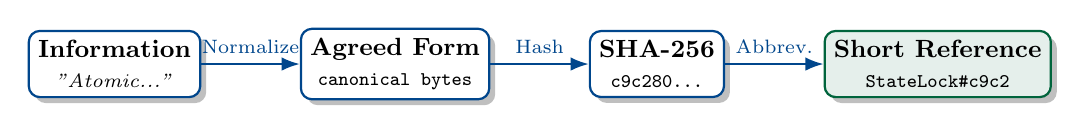
\begin{tikzpicture}[
    node distance=1.25cm,
    box/.style={rectangle, draw=semablue, thick, rounded corners, minimum height=0.8cm, align=center, fill=white, drop shadow, font=\small},
    arrow/.style={-Latex, thick, semablue}
]
    \node[box] (def) {\textbf{Information}\\ \textit{\scriptsize"Atomic..."}};
    \node[box, right=of def] (canon) {\textbf{Agreed Form}\\ \texttt{\scriptsize canonical bytes}};
    \node[box, right=of canon] (hash) {\textbf{SHA-256}\\ \texttt{\scriptsize c9c280...}};
    \node[box, fill=semagreen!10, draw=semagreen, right=of hash] (id) {\textbf{Short Reference}\\ \texttt{\scriptsize StateLock\#c9c2}};

    \draw[arrow] (def) -- node[above, font=\scriptsize] {Normalize} (canon);
    \draw[arrow] (canon) -- node[above, font=\scriptsize] {Hash} (hash);
    \draw[arrow] (hash) -- node[above, font=\scriptsize] {Abbrev.} (id);
\end{tikzpicture}
\caption{The content-addressing pipeline used in this paper. The digest is derived from an agreed representation and paired with a human-readable handle; the four-character form is a wire reference, while full-digest or full-root verification remains the security boundary. Other Sema realizations may use different representations and hash schemes.}
\label{fig:pipeline}
\end{figure}

The practical consequence is that a vocabulary of Pattern Cards behaves like an agent framework mixed into English. Agents can use as much structure as the moment requires, naming recurring mechanisms and leaving contextual prose freeform. When a recurring situation demands a different contract, an agent can mint a linked variant rather than paraphrase or overload the existing term. Once the relevant definitions are available, a few anchored words can replace repeated explanations of those definitions; Section~\ref{sec:token_compression} measures this wire-reference economy across five contract fields. It does not measure the preservation of every contextual detail when a whole passage is rewritten.

The same substrate can act as collective memory across summarization. Prose may shift at each compaction boundary, while a preserved full identifier remains pinned to the same verified definition for as long as its content remains resolvable. Sessions and agents can therefore retain stable conceptual anchors rather than relying only on surviving phrasing.

Pattern Cards offer three proposed channels of reasoning benefit. First, verified reference identity lets a conclusion cite the exact external definitions it used and exposes mismatch before work proceeds from a false shared assumption. Second, explicit invariants provide a mid-task checklist against which an agent or evaluator can test the work. Third, named procedures make often-implicit reasoning moves easier to request, combine, and revisit. These benefits depend on use: re-supplying an already clear definition may add context tokens without improving the result.

Models already produce fluent reasoning chains, and their fluency can allow unchecked premises to pass review. Pattern Cards are intended to make the steps explicit and enforceable by a surrounding workflow: citable by hash, checkable against a contract, and usable as inputs to a gate. The intended benefit lies in multi-step work, coordination, and long-horizon tasks rather than single-pass scoring over well-known material. Some of that benefit falls outside answer-only metrics: a verified refusal prevents an action or assertion rather than producing a scored answer.

The corrective-procedure intuition is familiar from human reasoning: a named move such as checking base rates, looking for survivorship bias, or seeking a counter-argument gives a reasoner a specific action to take. Pattern Cards extend this checklist idea into a resolvable vocabulary whose procedures are named, composable, and cumulatively revised. Their intended contribution to language-model reasoning is reliable access to such moves, not a claim that a model cannot infer an omitted step.

This is why the bootstrap library is closer in intent to a ``Constitution for a Digital City'' than a passive ``Library Catalog.'' Patterns such as \sema{LatticeCommit}{488a} and \sema{ReceptivityGate}{5667} specify how participants should handle integrity and admission, while reasoning cards specify moves an individual agent can invoke. The metaphor concerns explicit rules available for use and inspection; their authority, adoption, and enforcement remain decisions of the participating community.

\noindent\begin{minipage}{\textwidth}
This use is the first operational slice of a larger architecture: a Living Taxonomy of Thought. A Sema-equipped model could represent a book, theory, or strategy as a graph of referenced concepts, mechanisms, assumptions, and disagreements. Where an existing pattern fits exactly, the model reuses it; where the fit is only partial and the difference changes the concept's contract, it mints a linked variant rather than overloading the old word. Successive agents can therefore inherit not only documents, but an inspectable record of the conceptual distinctions extracted from them. Sema supplements rather than replaces the source material, and the resulting taxonomy need not be final: source-specific patterns may remain local, competing interpretations may coexist, and only broadly reusable concepts need enter a shared library. This paper implements the identity, resolution, composition, and minting substrate for that architecture; training models to construct and reason through work-scale pattern graphs remains future work.
\end{minipage}

%==============================================================================
\section{Problem Formalization}
\label{sec:formalization}

We use a minimal communication model to isolate the failure mode that motivates Sema; we do not attempt to formalize semantic equivalence in general. Let $\mathcal{A} = \{A_1, \ldots, A_n\}$ be a set of agents, where each agent $A_i$ maintains a local semantic model $M_i: \mathcal{L} \rightarrow \mathcal{S}$ mapping linguistic tokens $\mathcal{L}$ to internal semantic representations $\mathcal{S}$. When Agent~$A_i$ sends message $m \in \mathcal{L}$ to Agent~$A_j$, coordination is reliable only if:
\begin{equation}
M_i(m) \approx_\epsilon M_j(m)
\end{equation}
where $\approx_\epsilon$ denotes semantic equivalence within tolerance $\epsilon$. The failure mode is that agents cannot directly compare their private semantic mappings $M_i$ and $M_j$, so divergence accumulates silently until coordination breaks. Sema does not prove equality of internal representations. In the definition-coordination application developed here, full-reference verification instead establishes that agents resolved the same hashed external definition, independent of their private internal models.

A coordination mechanism for external semantic contracts must satisfy five key desiderata. \emph{Identity} (D1): agents can test whether two references denote the same canonical definition. \emph{Fail-Closed Coordination} (D2): mismatch blocks action rather than proceeding with different interpretations. \emph{Compactness} (D3): for nontrivial definitions, wire references should be smaller than the content they denote. \emph{Resolvability} (D4): a reference can be expanded or verified against the canonical object, without loss with respect to that canonical object (though not with respect to whatever private meaning an agent additionally attaches to it). \emph{Permissionless Minting} (D5): no central authority controls vocabulary creation.

%==============================================================================
\section{The Sema Protocol}
\label{sec:sema}
%==============================================================================

This section develops the representation and hashing rules, Pattern Card discovery (Section~\ref{sec:pattern_cards}), the fail-closed handshake (Section~\ref{sec:fail_closed}), and the type system used by the bootstrap library (Section~\ref{sec:type_system}).

\subsection{Design Principles}

Sema's core rule is representation-agnostic: hash information under an agreed representation and scheme, then use the resulting content address directly in communication. It is not restricted to JSON or to a fixed schema. Raw bytes, a canonical graph, or a structured object can each participate if recipients know how to resolve the reference and recompute its identity. The implementation used in this paper supplies deterministic recursive Merkle hashing for JSON-compatible objects; a molecular database, legal contract repository, or game-rule engine could define a different representation while retaining the same communication primitive.

The communication primitive, the JSON/Merkle realization, the Pattern Card schema, and the \emph{Sema Bootstrap Library} are distinct layers. Pattern Cards are this paper's concrete agent-coordination schema; the library in Section~\ref{sec:standard_library} is a bootstrapped opinion on useful definitions expressed through that schema. Coordination requires a shared Schelling point, so we provide \semaPatternCount~patterns designed to bootstrap agent society. Their fields describe actionable behavioral contracts rather than passive entries: the \texttt{mechanism} states the intended procedure, the \texttt{invariants} state what must remain true, and the \texttt{dependencies} state how a pattern composes. Execution and enforcement still require an agent, evaluator, implementation binding, or surrounding harness. What follows describes the JSON/Merkle mechanics and this concrete instantiation.

\subsection{Cryptographic Foundation}

Applied to definitions, the communication primitive permits a \emph{Semantic Commons}: a shared namespace where agents actively mint and reference new concepts without requiring a central authority to decide what words exist. Just as Git allows any developer to commit code, Sema allows any participant to mint a content-addressed item under an agreed representation. In this implementation, an agent defines a Pattern Card as a JSON object and computes its Merkle Root from the card's semantic fields, transforming the namespace from a read-only reference into a writable \emph{thoughtspace}.
\begin{equation}
    a_{\sigma}(x) = \text{Hash}_{\sigma}(\text{Encode}_{\sigma}(x))
\end{equation}
Here $\sigma$ identifies the agreed representation and hash scheme. The JSON/Merkle implementation specializes this rule to field-addressable Pattern Cards:
\begin{equation}
    H_{\text{pattern}} = \text{Merkle}(\{ \text{mechanism}, \text{gloss}, \text{dependencies}, \dots \})
\end{equation}
This hash becomes the permanent identity component for that object (e.g., \texttt{\#a1b2}); the readable handle remains separate. If Agent~A and Agent~B resolve the same full identifier, recompute the hash over the returned object, and obtain a match, they establish---subject to SHA-256 collision resistance---that they hold the same canonical definition, regardless of who created or stored it.

The JSON realization implements content-addressing via a Merkle Tree. Given a definition $d$ and a separate readable label $\ell$, the Pattern Card identifier is:
\begin{equation}
\text{id}(\ell,d) = \texttt{sema:} \| \ell \| \texttt{\#mh:SHA-256:} \| \text{RootHash}(d)
\end{equation}
where $\ell$ is not part of $\text{RootHash}(d)$, and $\text{RootHash}(d)$ is computed via recursive Merkle Tree construction using deterministic JSON canonicalization inspired by RFC 8785 (JSON Canonicalization Scheme)~\cite{rfc8785}, adapted with explicit NFC string normalization for deterministic string equivalence, and aligning with principles from RDF Dataset Canonicalization~\cite{longley2024rdf} and content-addressed semantic data~\cite{knowledgefutures2023}. This ensures that canonical-equivalent JSON objects produce deterministic hashes regardless of serialization order.

The current implementation uses canonicalization v2 (semahash 0.3.0), which domain-separates every Merkle node with an explicit type tag. Strings undergo NFC normalization followed by whitespace normalization and are hashed as $\text{SHA-256}(\mathrm{s:} \| \text{normalized UTF-8 text})$; primitive JSON values as $\text{SHA-256}(\mathrm{p:} \| \text{v2 primitive spelling})$; lists as $\text{SHA-256}(\mathrm{l:} \| H(L_1) \| H(L_2) \| \dots)$; and dictionaries as $\text{SHA-256}(\mathrm{d:} \| H(k_1) \| H(v_1) \| \dots)$, with entries sorted by normalized key and with normalized-key collisions rejected fail-closed. Dependency maps receive one additional canonicalization step: aliases are normalized through their target handles, and multiple aliases that intentionally reference the same handle are preserved as a sorted list rather than silently collapsed. These tags prevent structurally distinct JSON values---for example the string \texttt{"1"} and the number \texttt{1}, or a two-element list and a one-entry dictionary---from sharing the same hash input. The \href{https://github.com/emergent-wisdom/sema/blob/005f769735527d55a50d926afc054f5817b43d7e/docs/specification/schema.md\#4-the-hashing-protocol-normative-merkle-encoding}{normative encoding specification} defines the exact whitespace set, numeric spelling, lowercase ASCII-hex child digests, key ordering, and runtime compatibility boundaries; \href{https://github.com/emergent-wisdom/sema/blob/005f769735527d55a50d926afc054f5817b43d7e/docs/specification/canonicalization-v2-test-vectors.json}{interoperability vectors} supply exact preimages and rejection cases.

In the Pattern Card realization, dependency and specialization references, when present, carry their targets' full Sema IDs inside the hashed object. A card carrying such references therefore commits recursively to its exact referenced-definition closure, as cards in the bootstrap library do; the current implementation's aggregate roots below commit, independently of insertion history, to the vocabulary-wide definition set and handle bindings, but not to the mutable \texttt{\_meta} taxonomy. Neither referenced composition nor vocabulary-wide aggregate roots are requirements of the representation-agnostic Sema primitive.

Vocabulary snapshots require a second canonicalization layer because a set of disconnected pattern DAGs has no traversal-defined order. Beginning with semahash 0.4.0, the implementation therefore publishes two versioned commitments. The \emph{semantic-set root} commits to the sorted set of unique raw pattern digests; the \emph{catalog root} commits to the sorted mapping from each handle to its raw pattern digest. Both use scheme-specific leaf framing followed by the Merkle Tree Hash construction of RFC~9162~\cite{rfc9162}: leaves are $\text{SHA-256}(0x00 \| d)$, internal nodes are $\text{SHA-256}(0x01 \| L \| R)$, and a non-power-of-two list is recursively split at the largest power of two below its length. Thus an unpaired subtree is never duplicated. Sorting raw digests is the rule used here for unordered-set semantics---Certificate Transparency itself receives an already ordered log---while catalog entries are ordered by their handle bytes. The scheme identifier and leaf count accompany each root; a bare digest specifies neither its hash function nor its tree construction.

The per-pattern Merkle structure assigns every field a deterministic, collision-resistant hash, allowing agreement and disagreement to be localized even when full pattern roots differ. As a concrete example, suppose Agent~A and Agent~B both reference \sema{StateLock}{c9c2} but their pattern roots disagree. Field-level hash comparison may reveal matching \texttt{invariants} hashes (both definitions state that the lock is exclusive and auto-releases on timeout) while their \texttt{failure\_modes} hashes diverge (A's pattern enumerates network partition as recoverable; B's treats it as terminal). This identifies precisely which clauses match and which require reconciliation. Selective coordination on a matching subset requires an explicit policy; the current handshake remains fail-closed on root mismatch. Whole-document hashes (SDH, Agora, BlockA2A) collapse the comparison to a single binary mismatch, whereas the Pattern Card Merkle structure preserves field-level diagnostic granularity.

Crucially, the Pattern Card schema excludes metadata from identity. The \texttt{\_meta} object, containing fields like \texttt{path} (an ordered list of taxonomy segments such as \texttt{["Society", "Governance"]}), \texttt{tier}, \texttt{ring}, and \texttt{related}, is excluded from the hash calculation. This keeps taxonomy from becoming part of a pattern's permanent identity. The intuition is that the substrate is mathematics and the overlay is politics: equality of the hashed specification of what a pattern does is checked mathematically, while where it belongs remains mutable metadata subject to community judgment. This separation allows the community to reorganize categories, for instance by downgrading a pattern from Tier~1 to Tier~2 upon discovery of a vulnerability, without breaking the code of agents that rely on the pattern's hash; the identifier \sema{BayesUpdate}{11d2} remains valid even if its classification changes. The pattern identity is computed from eleven semantic fields:

\begin{center}
\begin{tabular}{ll}
\toprule
\textbf{Field} & \textbf{Purpose} \\
\midrule
\texttt{mechanism} & How the pattern works (the core definition) \\
\texttt{gloss} & Short definition (one-line summary) \\
\texttt{dependencies} & References to other patterns (the wiring) \\
\texttt{signature} & Type transformations, e.g., \texttt{Gate(Signal)} \\
\texttt{invariants} & Rules that must always hold \\
\texttt{preconditions} & Required state before invocation \\
\texttt{postconditions} & Required state after a valid invocation \\
\texttt{parameters} & Configurable parameter objects \\
\texttt{failure\_modes} & Known ways the pattern can fail \\
\texttt{data\_schema} & JSON Schema for runtime data structure \\
\texttt{extends} & Exact parent definition this specializes \\
\bottomrule
\end{tabular}
\end{center}

Fields not hashed include a pattern's own \texttt{handle}, \texttt{\_meta}, and any \texttt{sema\_*} fields. Reclassification therefore leaves identity unchanged, and renaming a pattern does not change that pattern's own digest. Canonicalization v2 does, however, retain target handles inside hashed structured references: dependency maps contain target handles, and \texttt{extends} stores a full Sema ID. Renaming a referenced pattern can therefore change the hashes of both dependents and specialized descendants; graph-wide rename invariance requires a separate versioned canonicalization migration covering both forms. For backward verification, a pre-0.4 card carrying the former \texttt{derived\_from} key is hashed under that original key and is not reinterpreted as an \texttt{IS\_A} claim; explicit migration to \texttt{extends} produces a new identity.

For human readability, prose references use a 4-character stub of the root hash, such as \sema{PropheticQuorum}{fb6b}; full dependency fields and security-sensitive handshakes retain or resolve the full hash or compare the relevant aggregate root. To keep mechanism text independently comparable as dependencies evolve, the implementation uses a template hashing strategy where the mechanism uses local placeholders like \texttt{\{\{hypothesis\}\}} representing the algorithm, while the wiring maps these placeholders to specific hashes in the \texttt{dependencies} object. The Pattern Identity is the Merkle Root of both, allowing tools to distinguish a logic-field match from a dependency-wiring mismatch when agents use different library versions. Rewiring can change the procedure's behavior even when its mechanism text is unchanged.

\subsection{Discovery and Pattern Cards}
\label{sec:discovery_loop}
\label{sec:pattern_cards}

The Pattern Card tooling reconciles two opposing needs: discovery, which benefits from ambiguity and high recall, and coordination, which requires exact identity for the references being verified. It does so through \emph{progressive ambiguity collapse}, captured by the \sema{Taper}{bebf} pattern: discovery begins broadly, then the workflow narrows to selected definitions whose identities can be checked exactly. First, in the \emph{Orient} phase, the agent queries the topology via \texttt{sema\_graph\_skeleton()} to obtain a low-resolution map of regions and hubs. Next, during \emph{Explore}, the agent performs a hybrid search merging field-weighted keyword matches (handle: 1.0, signature: 0.75, gloss: 0.70, mechanism: 0.55) with vector embeddings (Score 0.3--0.7). This strategy mirrors Blended RAG~\cite{sawarkar2024blended}, merging keyword precision with semantic recall~\cite{arivazhagan2023}. However, reliance on fuzzy search alone is hazardous; audits of encyclopedic search engines reveal that they frequently surface content only ``weakly related'' to the query~\cite{coppolillo2025unexpected}. This hybrid strategy allows approximate intent (e.g., ``how to handle errors'') to find precise patterns (e.g., \sema{Retry}{4f9f}), but necessitates the subsequent verification step. Finally, in the \emph{Verify} phase, the agent invokes \texttt{sema\_handshake()} (Section~\ref{sec:fail_closed}), which distinguishes cooperative drift detection from strict identity verification. The pipeline uses semantic similarity for discovery and hash-based identity comparison for coordination.

\begin{figure}[h]
\centering
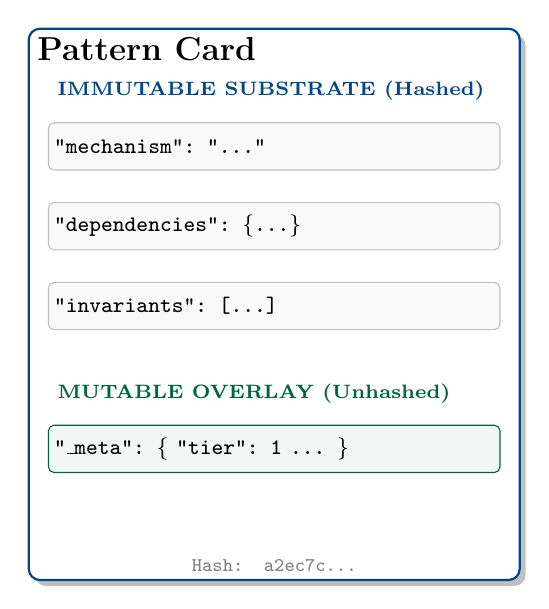
\begin{tikzpicture}[
    card/.style={rectangle, draw=semablue, thick, rounded corners=4pt, fill=white, drop shadow, text width=6cm, font=\small},
    field/.style={rectangle, draw=gray!50, rounded corners=2pt, fill=gray!5, text width=5.5cm, minimum height=0.6cm, font=\footnotesize\ttfamily},
    label/.style={font=\scriptsize\bfseries, text=semablue, anchor=west}
]
    \node[card, minimum height=7cm] (main) {};

    \node[anchor=north west, font=\bfseries\large] at (main.north west) {Pattern Card};

    % Immutable Substrate (Hashed)
    \node[field, anchor=north] (mech) at ($(main.north)+(0,-1.2)$) {"mechanism": "..."};
    \node[label] at ($(mech.north west)+(0,0.4)$) {IMMUTABLE SUBSTRATE (Hashed)};
    \node[field, anchor=north] (dep) at ($(mech.south)+(0,-0.4)$) {"dependencies": \{...\}};
    \node[field, anchor=north] (inv) at ($(dep.south)+(0,-0.4)$) {"invariants": [...]};

    % Mutable Overlay (Unhashed)
    \node[field, anchor=north, draw=semagreen, fill=semagreen!5] (meta) at ($(inv.south)+(0,-1.2)$) {"\_meta": \{ "tier": 1 ... \}};
    \node[label, text=semagreen] at ($(meta.north west)+(0,0.4)$) {MUTABLE OVERLAY (Unhashed)};

    % Hash
    \node[anchor=south, font=\ttfamily\scriptsize, text=gray] at (main.south) {Hash: a2ec7c...};

\end{tikzpicture}
\caption{Pattern Card Anatomy. The \emph{Substrate} defines identity (hashed); the \emph{Overlay} enables evolution (unhashed).}
\label{fig:anatomy}
\end{figure}

A Sema Pattern is not merely a dictionary definition; it is a structured behavioral specification (Figure~\ref{fig:anatomy}). Preconditions, postconditions, and invariants make contract clauses explicit for inspection by agents, external evaluators, or executable bindings; the Pattern Card does not itself execute or enforce them. This structure builds on a lineage of structured LLM frameworks---notably DSPy Signatures~\cite{khattab2024dspy}, DSPy Assertions~\cite{singhvi2024dspy}, and the Prompt Pattern Catalog~\cite{white2023prompt}---which introduced contract-like constraints for language model pipelines. Sema's contribution is to make canonical contract identity hash-verifiable: including the clauses in the Merkle root permits cached digest comparison without asking a model whether two contract texts mean the same thing. We selected these fields to transform vocabulary from \emph{Passive Knowledge} into explicit contract structure, as illustrated by the schema for \sema{PropheticQuorum}{fb6b}:

\Needspace{8\baselineskip}
\begin{description}
    \item[Dependencies (The Imports)]
    \textbf{Rationale:} A categorized map of hard links. Makes declared dependencies machine-readable without parsing natural language.\\
    \textbf{Example:}
    \begin{lstlisting}[numbers=none]
"dependencies": {
  "composes_with": {
    "sim": "sema:Simulation#mh:SHA-256:1058e7090079e846251ed480d7afec0328809d22bebb6b205425b2de614787c3",
    "vote": "sema:Vote#mh:SHA-256:84935dbc846bcd8fe2da01e9e04401f190769e87d0354e00c0986e43e414f300"
  },
  "accepts": {
    "proposal": "sema:Proposal#mh:SHA-256:5d0a98055eef6c963d4c9ec0403cac243720ce8927398032c19b4f5d8cc94506"
  },
  "yields": {
    "decision": "sema:Decision#mh:SHA-256:b1407127acd4a39314fc24b418310e4b95e0347e4e22f376151ab765e2dfd2c7"
  }
}
    \end{lstlisting}

    \item[Mechanism (The Procedure)]
    \textbf{Rationale:} Describes the intended procedure using the keys defined in Dependencies.\\
    \textbf{Example:} ``Instantiates \texttt{\{\{sim\}\}} to predict outcomes of \texttt{\{\{proposal\}\}} before calling \texttt{\{\{vote\}\}} to produce \texttt{\{\{decision\}\}}.''

    \item[Invariants (The Safety Contract)]
    \textbf{Rationale:} States conditions that must hold throughout a valid application; checking them requires an agent, evaluator, or executable binding.\\
    \textbf{Example:} ``Prediction Precedence: Vote must occur after Simulation.''

    \item[Preconditions (Entry Conditions)]
    \textbf{Rationale:} Records conditions that must hold before application, supporting chaining and planning when an agent or external evaluator checks them.\\
    \textbf{Illustrative example:} ``The input state and simulation configuration have been fixed before invocation.'' A precondition such as ``Determinism level is high'' additionally needs an agreed criterion for ``high.''

    \item[Gloss (The Embedding Anchor)]
    \textbf{Rationale:} A semantic hook for vector retrieval.\\
    \textbf{Example:} ``Aligning predictions before aligning votes.''

    \item[Specialization (The Type Relation)]
    \textbf{Rationale:} Records that this definition is a narrower kind of an exact parent definition and emits an \texttt{IS\_A} edge.\\
    \textbf{Example:} \texttt{"extends": "sema:Task\#mh:SHA-256:..."}. Because the parent version is named by its full identifier, retargeting the child is an explicit semantic change.

    \item[Metadata (The Overlay)]
    \textbf{Rationale:} Stores the evolving knowledge graph (associations, suggestions, safety tiers) without affecting the identity hash.\\
    \textbf{Example:} \texttt{"\_meta": \{ "tier": 1, "related": ["Mutex\#b031"], "supersedes": ["sema:OldHandle\#mh:SHA-256:..."] \}}. The unhashed \texttt{supersedes} list records version history without making the route by which a definition was authored part of its identity.
\end{description}

\subsection{The Fail-Closed Protocol}
\label{sec:fail_closed}

When agents coordinate using Sema patterns, the MCP tool \texttt{sema\_handshake} compares the selected external definitions required for the interaction (the ``Context''). The initiating agent lists the required pattern identifiers; each agent independently resolves them and deterministically constructs the catalog Merkle Tree of that subset. Each leaf binds a requested handle to the hash of the definition it resolved, so swapping two handles' definitions cannot preserve the root. The agents exchange the declared root scheme and full Merkle Root:

\begin{equation}
R_{context} = \text{CatalogMerkleRoot}(\{(h_1,\hash(d_1)), (h_2,\hash(d_2)), \dots, (h_n,\hash(d_n))\})
\end{equation}

Matching full roots and schemes establish, subject to collision resistance, that every selected handle resolved to the same canonical definition and hence the same external contract. A strict, enforced handshake permits coordination with short references on a match and halts immediately on either root or scheme mismatch (Figure~\ref{fig:handshake}). Enforcement belongs to the execution harness: it must require and honor the handshake. The guarantee covers \emph{compliant} agents; the protocol alone supplies no Byzantine guarantee. If active attackers are in scope, comparison requires authenticated references or transport. A deployment can additionally require handshake tokens at message admission, rejecting non-compliant agents' messages at that boundary. Integrating these enforcement boundaries is a deployment decision (Section~\ref{sec:limitations}).

The current convenience tools \texttt{sema\_propose\_context} and \texttt{sema\_verify\_context} exchange an eight-hex-character catalog-root prefix and label it explicitly as cooperative drift detection, not adversarial security; they require the declared scheme even in this mode. A full semantic-set root answers the weaker question of whether the raw definition-digest sets match; under canonicalization v2, those digests can still change when target handles in structured references are renamed.

\begin{figure}[H]
\centering
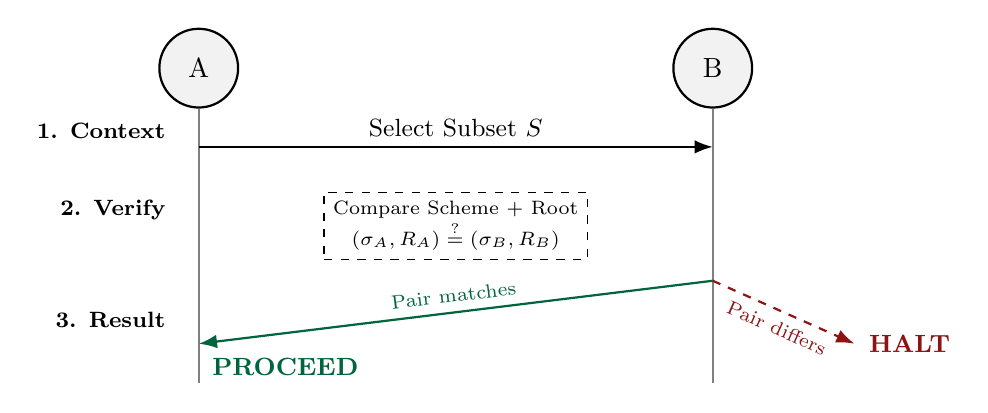
\begin{tikzpicture}[
    node distance=2.5cm,
    agent/.style={circle, draw=black, thick, minimum size=1cm, fill=gray!10},
    msg/.style={font=\small\ttfamily}
]
    % Agents
    \node[agent] (A) {A};
    \node[agent, right=5.5cm of A] (B) {B};

    % Timeline
    \draw[thick, gray] (A) -- ++(0,-4);
    \draw[thick, gray] (B) -- ++(0,-4);

    % Step 1: Context
    \node[anchor=east, font=\footnotesize\bfseries] at (-0.3,-0.8) {1. Context};
    \draw[-Latex, thick] ($(A)+(0,-1)$) -- node[above, msg, font=\small] {Select Subset $S$} ($(B)+(0,-1)$);

    % Step 2: Verify
    \node[anchor=east, font=\footnotesize\bfseries] at (-0.3,-1.8) {2. Verify};
    \node[draw, dashed, align=center, fill=white, font=\scriptsize] at ($(A)!0.5!(B) + (0,-2)$) {Compare Scheme + Root\\$(\sigma_A,R_A) \stackrel{?}{=} (\sigma_B,R_B)$};

    % Step 3: Branch
    \node[anchor=east, font=\footnotesize\bfseries] at (-0.3,-3.2) {3. Result};
    \draw[-Latex, semagreen, thick] ($(B)+(0,-2.7)$) -- node[above, sloped, font=\scriptsize] {Pair matches} ($(A)+(0,-3.5)$);
    \node[text=semagreen, font=\small\bfseries] at ($(A)+(1.1,-3.8)$) {PROCEED};

    \draw[-Latex, semared, thick, dashed] ($(B)+(0,-2.7)$) -- node[below, sloped, font=\scriptsize] {Pair differs} ($(B)+(1.8,-3.5)$);
    \node[text=semared, font=\small\bfseries] at ($(B)+(2.5,-3.5)$) {HALT};
\end{tikzpicture}
\caption{Fail-closed handshake. Agents compare the root scheme and Merkle Root of the agreed pattern subset; an enforced handshake maps divergence in either to \texttt{HALT}.}
\label{fig:handshake}
\end{figure}

This represents a deliberate inversion of Postel's Law~\cite{postel1980}. Where the Internet's robustness principle advises ``be liberal in what you accept,'' Sema inverts the receiving side: be strictly conservative in what you accept, and reject what you cannot verify. This choice prioritizes safety over permissive interoperability: compliant deployments reject mismatches in the selected external definitions rather than interpreting them on a best-effort basis. In multi-agent systems where definitional drift can cascade into consequential failure, an explicit fail-closed boundary is valuable.

\begin{proposition}[Canonical Hash Collision Bound]
Under the standard random-oracle approximation, for a vocabulary of size $|\vocab|$ the probability of two distinct canonical definitions producing the same SHA-256 digest is bounded by:
\begin{equation}
P(\text{collision}) \leq \frac{|\vocab|^2}{2^{257}} \approx 0
\end{equation}
\end{proposition}

This follows from the birthday bound under the stated random-oracle approximation. With $|\vocab| = \semaPatternCount$, collision probability is negligible ($< 10^{-72}$).

\begin{proposition}[Strict Fail-Closed Detection]
If agents $A_i$ and $A_j$ resolve distinct canonical definitions $d_i$ and $d_j$ for pattern $P$, then $\hash(d_i) \neq \hash(d_j)$ with overwhelming probability. A strict, enforced handshake comparing full digests or full roots therefore halts for compliant agents; cooperative prefix mode provides drift detection only. Adversarial deployments additionally require authenticated references or transport.
\end{proposition}

\begin{proposition}[External Contract Identity]
If agents $A_i$ and $A_j$ both resolve a full identifier $I$ against an honest content-addressed store, obtain canonical definitions $d_i$ and $d_j$, and verify $\hash(d_i)=\hash(d_j)=\operatorname{digest}(I)$ under the same agreed representation and hash scheme, then $d_i=d_j$ subject to hash collision resistance. They therefore hold an identical \emph{external} semantic contract for $I$, independent of their private internal semantic models $M_i, M_j$. Sema does not prove $M_i(I) = M_j(I)$; it establishes identity of the externally resolved object under these assumptions, so any divergence in downstream behavior cannot be attributed to the agents having resolved different definitions under that identifier.
\end{proposition}

\begin{proposition}[Compression with Resolvable Expansion]
Let $|r|$ be reference length (handle + 4-char hash $\approx$ 15 characters) and $|d|$ be definition length. Compression ratio is $|d|/|r|$. Given a declared resolver or catalogue in which $r$ maps unambiguously to $d$, expansion is deterministic. Cryptographic assurance still requires verification against the full pattern hash or an agreed context or aggregate root; the short stub is a readable locator, not a self-authenticating security boundary.
\end{proposition}

\subsection{The Type System}
\label{sec:type_system}
\label{sec:wiring}
\label{sec:compiler}

This is the bootstrap library's \emph{particular} type system; other schemas
remain possible. Field-level interoperability and resolution require shared
schemes, and the current registry and handshake tools implement the Pattern
Card case. Sema is closer to Unicode than to a universal language: it
standardizes a way to carry identity, not every vocabulary spoken through it.

We chose the agent-protocol schema below because structural typing lets the same
verb operate across domains as long as subjects satisfy a common contract, and
polymorphic dispatch lets an agent request ``any pattern that implements
Deep(Discover)'' rather than pinning a specific hash. Readers interested only in
protocol-level guarantees may skip to Section~\ref{sec:standard_library};
readers interested in how this schema handles polymorphism, composition, and wiring
across \semaPatternCount{}~patterns should continue here.

A central tension in vocabulary design is determining when a change in attributes constitutes a change in identity. The bootstrap library adopts a structural resolution: qualitative differences create distinct patterns, while quantitative differences create parameters with hashed range contracts. For example, \sema{ExponentialBackoff}{f5e5} with a \texttt{base\_delay} of 100ms and the same pattern with a 5-second delay share the same Pattern-definition identity because the hash captures the parameter range contract, not the instance value. However, if changing a variable alters the failure mode, such as switching from busy-waiting to database storage, it becomes a distinct pattern (e.g., \texttt{SpinLock} vs. \texttt{Lease}). This declares a range against which a surrounding runtime may validate instance values while preserving one pattern definition.

To support open-ended reuse without creating incompatible ad hoc interfaces, the Pattern Card schema employs Typed Interfaces. The \texttt{dependencies} object partitions declared aliases among four roles: \texttt{accepts} defines passive input data patterns consumed by the mechanism; \texttt{yields} defines passive output data patterns produced by the mechanism; \texttt{composes\_with} defines active tool or logic patterns explicitly invoked by the mechanism; and \texttt{references} defines patterns used for conceptual clarity but not execution. Each alias occurs in exactly one category, making this map the ``Single Source of Truth'' for dependency wiring. The separate \texttt{extends} field records specialization. Acyclicity is enforced by a separate graph check over both dependency and specialization links, yielding a directed acyclic graph (DAG).

Typed interfaces decouple verbs from specific noun instances. A LogisticsAgent locking a shipping container and a MedicalDrone locking a patient record can both invoke the same pattern when both subjects satisfy the \texttt{accepts} interface (e.g., \texttt{"accepts": \{ "subject": "sema:UniqueHandle..." \}}). In this example, the agent or runtime must check each subject against the referenced \texttt{UniqueHandle} contract; a noun's \texttt{data\_schema}, when provided, makes its structural constraints explicit. Compatibility depends on the declared contract rather than variable names. This architecture allows the \semaPatternCount~core patterns to support many cross-domain compositions through shared noun definitions.

The integrity of these compositions is enforced by the Explicit Wiring Rule, which welds the abstract type to the concrete logic. The compiler mandates that every element in a pattern's \texttt{signature} (the claim, e.g., \texttt{Check(Safety)}) must be explicitly imported in the \texttt{dependencies} and invoked in the pattern's text fields (mechanism, invariants, preconditions, postconditions, or failure modes) via a template key. An accepted Pattern Card therefore cannot declare a signature without the required links in its hashed specification; this validates the card's wiring, not the behavior of an eventual implementation.

The Pattern Card tooling resolves these high-level intents into concrete pattern handles. When an agent submits a polymorphic intent such as \texttt{Deep(Discover)}, the registry resolver looks for that exact declared signature (e.g., on \sema{DeepResearch}{c1f1}) and returns the selected card with its dependency subgraph to the requested depth. The current \href{https://github.com/emergent-wisdom/sema/blob/005f769735527d55a50d926afc054f5817b43d7e/src/sema/core/registry.py\#L916}{resolver} selects the first matching entry in registry iteration order; no match produces a not-found result. Different registries can therefore select different implementations of the same intent. Coordination verifies the resulting concrete full identifiers or context root (Section~\ref{sec:fail_closed}), rather than treating the signature alone as a shared definition. This resolution step decouples intent from a specific pattern definition, allowing the system to retarget the underlying procedure, such as swapping a heuristic check for a rigorous crypto-audit, without altering the agent's cognitive script. Executing the resolved procedure still requires an agent or implementation binding.

\begin{table}[h]
\centering
\caption{The Deep Registry: Resolving Polymorphic Rigor. Fast and Slow refer to lightweight versus heavyweight resolution strategies.}
\label{tab:deep_registry}
\begin{tabular}{@{}lll@{}}
\toprule
\textbf{Intent (Query)} & \textbf{Source Pattern (Fast)} & \textbf{Resolved Target (Slow)} \\ \midrule
\texttt{Deep(Heuristic)} & \sema{HeuristicSnap}{b95f} & \sema{MentalSim}{1ca0} \\
\texttt{Deep(Trace)} & \sema{Trace}{b68d} & \sema{GenealogicalTrace}{ee20} \\
\texttt{Deep(Discover)} & \sema{Discover}{f6e0} & \sema{DeepResearch}{c1f1} \\
\texttt{Deep(Nature)} & \sema{Nature}{9ac1} & \sema{LivedProof}{4aa1} \\ \bottomrule
\end{tabular}
\end{table}

At the wire level, the hash functions as a word in the natural-language stream that agents exchange; the LLM does not reason directly over hash bytes. To use the referenced procedure, an agent or host runtime resolves the definition and places the relevant text in model context. The deployment pattern assumed here is:
\begin{equation}
\text{Prompt} = \text{System} \oplus \text{Hydrate}(\text{Patterns}) \oplus \text{Query}
\end{equation}
The \emph{wire-level token}, such as \texttt{PropheticQuorum\#fb6b}, stays compact in communication; its resolved definition occupies model context. The design thus trades context-window tokens for wire-level integrity, with assurance supplied by full-identifier or agreed-root verification.

%==============================================================================
\section{The Bootstrap Library}
\label{sec:standard_library}

This section presents the Sema Bootstrap Library: the Schelling-point vocabulary introduced in Section~\ref{sec:sema}. The library is an initial seed rather than a closed canon; if an agent requires a different locking mechanism, it can permissionlessly mint a distinct variant such as \texttt{LeaseStateLock} without breaking the protocol.

\subsection{Methodology}

The initial vocabulary is a pragmatic bootstrap assembled without a principled
selection procedure. A different author could produce a different vocabulary
using the same protocol; the protocol's value is independent of any particular
library. The \semaPatternCount~patterns emerged iteratively from four sources:
distributed-systems primitives, the cognitive-decomposition architecture
developed in~\cite{westerberg2026crp}, model-assisted gap analysis, and the
author's domain analysis of agent failure modes. Creativity protocols such as
Adversarial Evolutionary Generation~\cite{westerberg2026alien} were used for
some frontier patterns.

The process became more structured as the library grew. Refinement checkpoints
used a dedicated ``Taxonomist'' role to reject duplicates, merge overlapping
concepts, and enforce the Noun/Verb separation; repeated failures became rules
and guidelines (Section~\ref{sec:refinement}). Structural validation is required
before \texttt{sema apply} mutates the vocabulary; Section~\ref{sec:implementation}
details those gates. Separate corpus audits report similarity, redundancy,
and contract-field coverage as advisory evidence for Taxonomist review and
human adjudication.

Admission to the bootstrap library requires at least one of two curation
criteria. A concept earns a pattern if it requires \emph{protocol consistency}---
multiple agents must coordinate on the exact semantics, as with
\sema{StateLock}{c9c2}---or if specifying it produces
\emph{structured thinking}, forcing a loosely used English concept into an
invariant-bearing mechanism. English suffices when neither criterion is met.
Pattern \emph{generality} is then reviewed through a broad-use test: compare
legitimate deployment contexts, retain the mechanism and invariants they share,
and place context-specific requirements in descendants via \texttt{extends}.
For example, \sema{Task}{a850} specifies recursive intent and inherited
constraints, while \sema{BoundedTask}{86dd} adds an explicit budget enclosure and
quality gate. The \sema{Lock}{95c2} $\rightarrow$ \sema{Mutex}{b031} family
likewise preserves the general exclusion contract while specifying a concrete
ownership mechanism. This review seeks a useful intersection: broad enough to
support legitimate variants and concrete enough to constrain behavior. It does
not exhaust every possible deployment context.

After the refinement pass described in Section~\ref{sec:refinement}, the
applied audits detect no duplicate mechanism strings, canonical-form duplicates,
or hash collisions across \semaPatternCount{}~patterns. Embedding-similarity
sweeps provide a further screen for near-duplicates
(Table~\ref{tab:embeddings}). These audits and Taxonomist review support library
quality, but they do not guarantee functional uniqueness
(see §\ref{sec:limitations}, ``The Synonymy Limit''). We make no claim to
completeness or optimality.

\subsection{The Civilization Stack}

The vocabulary is not a flat list; it is structured into four fundamental layers mimicking a civilization stack. At the base lies \textbf{Physics}, substrate primitives that obtain independently of any author (e.g., \sema{Lock}{95c2}, \sema{Entropy}{d5f7}, \sema{Gradient}{ecfc}, \sema{Equilibrium}{4f03}, \sema{Conservation}{0b32}, \sema{Distance}{dfdf}, \sema{PhaseTransition}{b775}, \sema{Attractor}{0036}, \sema{MutualInformation}{e714}, and \sema{Measurement}{511d}). Above this rests \textbf{Mind}, mechanisms that structurally require cognition (e.g., \sema{BayesUpdate}{11d2}), where judgment must be exercised and a single isolated agent can execute the mechanism. Emerging from these is \textbf{Society}, mechanisms that structurally require $\geq 2$ independent parties with potentially divergent state (e.g., \sema{Consensus}{b9a5}). Enclosing all three is \textbf{Infrastructure} (Figure~\ref{fig:stack}): authored structures and operations that do not require cognition to execute---data types, composite topologies, and mechanical operations (e.g., \sema{Mutex}{b031}).

The placement of each pattern is governed by the \emph{mechanism-sufficiency test}: what does the pattern's mechanism structurally require to execute? A pattern whose mechanism requires nothing more than substrate goes to Physics; one that requires authored structure but no cognition goes to Infrastructure; one that requires cognition but can be executed by a single isolated agent goes to Mind; one that structurally requires another party with separate state goes to Society. Placement follows the mechanism's execution requirements rather than its typical application domain or subject matter. This test is the governing principle recorded in \href{https://github.com/emergent-wisdom/sema/blob/main/docs/core/philosophy.md}{\texttt{docs/core/philosophy.md~\S3.1}}.

The four-layer ordering is a design discipline for this bootstrap library; other semantic vocabularies may use different decompositions. Its motivation is operational rather than ontological: lower layers should not depend on higher layers because doing so makes mechanical guarantees depend on social or cognitive assumptions. Resource and execution guarantees should not depend on reasoning strategies or social protocols, while social protocols may safely depend on lower-level execution and reasoning primitives. The ``Semantic Inversion Attack'' analyzed in §\ref{sec:hardening} illustrates the dependency error this discipline rejects.

\begin{figure}[h]
\centering
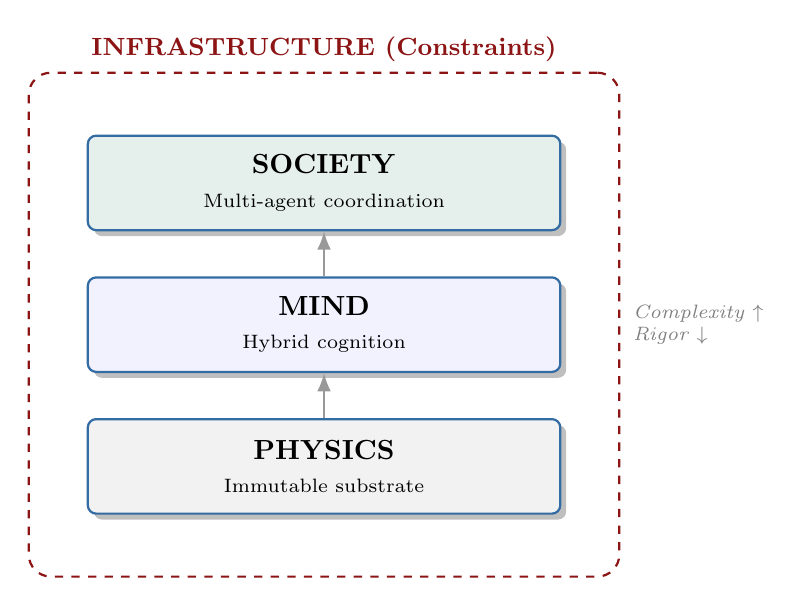
\begin{tikzpicture}[
    layer/.style={rectangle, draw=semablue!80, thick, minimum width=6cm, minimum height=1.2cm, align=center, rounded corners=3pt, fill=white, drop shadow},
    constraint/.style={rectangle, draw=semared, dashed, thick, minimum width=7.5cm, minimum height=6.4cm, align=center, rounded corners=8pt},
    label/.style={font=\scriptsize\sffamily, text=gray}
]
    % Infrastructure as container
    \node[constraint] (infra) at (0,0) {};
    \node[anchor=south, font=\small\bfseries, text=semared] at (infra.north) {INFRASTRUCTURE (Constraints)};

    % Stack inside
    \node[layer, fill=semagreen!10] (society) at (0,1.8) {\textbf{SOCIETY}\\{\scriptsize Multi-agent coordination}};
    \node[layer, fill=blue!5] (mind) at (0,0) {\textbf{MIND}\\{\scriptsize Hybrid cognition}};
    \node[layer, fill=gray!10] (physics) at (0,-1.8) {\textbf{PHYSICS}\\{\scriptsize Immutable substrate}};

    % Arrows
    \draw[-Latex, thick, gray!80] (physics.north) -- (mind.south);
    \draw[-Latex, thick, gray!80] (mind.north) -- (society.south);

    % Side annotations
    \node[anchor=west, font=\scriptsize\itshape, text=gray, align=left] at (3.8, 0) {Complexity $\uparrow$\\Rigor $\downarrow$};
\end{tikzpicture}
\caption{The Civilization Stack. Physics supports Mind, which enables Society; arrows show support from lower to upper layers. Infrastructure encloses this conceptual stack as authored constraints and operations. The bootstrap's separate hard-dependency ordering is Society $\rightarrow$ Mind $\rightarrow$ Physics $\rightarrow$ Infrastructure, with same-layer dependencies also permitted.}
\label{fig:stack}
\end{figure}

This stratification supports a property similar to Stewart Brand's ``Pace Layering''~\cite{brand1999clock}: lower layers provide stability for the turbulence of upper layers. Separating \textbf{Physics} primitives such as \sema{Entropy}{d5f7} from \textbf{Society} agreements such as \sema{Constitution}{3deb} allows social contracts and voting protocols to change without redefining lower-layer terms. The layer discipline therefore reduces coupling between governance and substrate guarantees.

The dependency graph must form a DAG because recursive dependency hashing
requires an acyclic order; the validator rejects cycles. Layer direction is a
separate library policy: an acyclic graph can still contain a dependency from a
mechanical primitive to a social agreement. Because layer metadata is excluded
from the hash, a card's identity depends on its canonical specification and
references, while its filing tier remains mutable. Libraries can therefore
adopt different layer policies and retain hash-level interoperability when
they share the Pattern Card scheme.

The bootstrap library applies a stricter policy (Section~\ref{sec:refinement}): hard dependencies (\texttt{accepts}, \texttt{composes\_with}) must remain within the same layer or flow to a more fundamental layer (Society $\rightarrow$ Mind $\rightarrow$ Physics $\rightarrow$ Infrastructure), enforced as a \texttt{sema apply} gate, while soft citations (\texttt{references}) and outputs (\texttt{yields}) are exempt and allow semantically necessary cross-layer links (for example, \sema{Belief}{e160} in Infrastructure soft-references \sema{Agent}{e127} in Mind because beliefs are conceptually held by agents, and the reference is acyclic). The current vocabulary contains \semaPatternCount~patterns organized into \semaCategoryCount~categories across these four layers (Table~\ref{tab:categories}; complete taxonomy in Appendix~\ref{app:taxonomy}), with zero patterns violating the layer-direction rule at this version.

\begin{table}[t]
\centering
\caption{Bootstrap library: \semaPatternCount~patterns across \semaCategoryCount{} category names and 4 layers}
\label{tab:categories}
\small
\begin{tabular}{llcp{3.8cm}}
\toprule
\textbf{Layer} & \textbf{Category} & \textbf{N} & \textbf{Examples} \\
\midrule
\multirow{2}{*}{Physics}
& Primitives & 16 & Attractor, Causation, Conservation \\
& Time & 1 & CausalBarrier \\
\midrule
\multirow{3}{*}{Infrastructure}
& Data Structures & 96 & AcceptSpec, Aesthetics, Anomaly \\
& Primitives & 52 & Act, Actor, Aggregate \\
& Verification & 9 & AuditTrail, CompatibilityCheck, ExplainBeacon \\
\midrule
\multirow{4}{*}{Mind}
& Inference & 22 & BaseRateInclude, BayesUpdate, BreadthGovernor \\
& Memory & 15 & BeliefTracking, ChunkMerge, ContextCompress \\
& Reasoning & 61 & Abduction, BackwardChain, Bisect \\
& Strategy & 81 & AdversarialSteel, Agent, AnalogyBridge \\
\midrule
\multirow{4}{*}{Society}
& Coordination & 12 & Compromise, Consensus, ConsensusFinder \\
& Economics & 9 & AtomicBid, AttentionMarkets, Award \\
& Governance & 7 & AnchorDrop, Constitution, DocumentedOverride \\
& Protocols & 75 & AdversarialProof, AgentDiscover, AgentProtocol \\
\midrule
& \textbf{Total} & \textbf{456} & \\

\end{tabular}
\end{table}
\FloatBarrier

\subsection{The Grammar of Agency}
\label{sec:grammar}
\label{sec:data_layer}
\label{sec:overlay_graph}

The vocabulary is not a flat list of tools but a compositional grammar that enables agents to construct novel intents from atomic units. \emph{Primitives} act as the fundamental building blocks of agent cognition. Five foundational verbs map to dimensions of autonomous inquiry: \sema{Discover}{f6e0} (Breadth) acts as the Scout, querying the horizon to find new nodes, agents, or paths; \sema{Deep}{16b0} (Depth) serves as the Scientist, escalating from heuristic proxies to rigorous implementations; \sema{Trace}{b68d} (Time) functions as the Historian, reconstructing causal chains within the records it holds; \sema{Check}{6890} (Validity) operates as the Critic, filtering inputs against invariants; and \sema{Stigmergy}{dd4f} (Space) works as the Builder, writing persistent signals for indirect coordination. Alongside these verbs, noun primitives such as \sema{Belief}{e160}, \sema{Agent}{e127}, and \sema{Constraint}{7013} provide the objects of agency.

These primitives enable a higher-order grammar where complex behaviors compose from atomic units: \sema{Check}{6890}(Condition) evaluates a target \sema{Condition}{b480} and yields Verified, Falsified, or Unknown without changing control flow; \sema{Trace}{b68d}(Target) wraps a process to generate an immutable lineage log whose coverage may be partial; and \sema{Stigmergy}{dd4f}(Signal) marks the shared environment with a signal for others to discover.

\emph{Macros} are composite patterns built from primitives via semantic import.
These grammatical roles describe how patterns compose; they are separate from
the library's mutable ring assignments and its safety-rigor tiers
(Tier~1--3, Section~\ref{sec:contract_levels}). Both metadata classifications
live in the unhashed overlay. For example,
\sema{AgentDiscover}{b784} imports \texttt{\{\{Discover\#f6e0\}\}} acting on
\texttt{\{\{Agent\#e127\}\}}, while \sema{TraceBelief}{7ccc} imports
\texttt{\{\{Trace\#b68d\}\}} acting on \texttt{\{\{Belief\#e160\}\}}.
This grammar allows agents to express intent via queries like ``I need to
\texttt{Deep(Trace)} this belief,'' which the resolution workflow described in
Section~\ref{sec:type_system} connects to concrete pattern definitions.

This distinction reveals a bicameral architecture. Primitives serve as the
query interface, allowing agents to identify logical gaps in the vocabulary.
Macros like \sema{IdentityHandshake}{4397} serve as the social interface,
enabling efficient coordination through compression. A verified Macro identity
commits to its imported components, so agents can establish one composite
agreement covering several primitives. This can reduce exchanges in workflows
that would otherwise negotiate those components separately. Primitives are for
querying; Macros are for talking.

The verb/noun distinction introduced in the Type System (Section~\ref{sec:type_system}) also addresses the ``schema drift'' problem where implicit schemas lead to subtle incompatibilities. Pattern Cards formalize the ``shape of work'' as content-addressed Data Patterns. \sema{Task}{a850} represents a recursive definition of intent that inherits constraints from its parent and explicitly defines its \texttt{AcceptSpec}. \sema{Solution}{8d55} acts as a container for work product, encapsulating provenance and, for composite work, a component tree for supply-chain auditing. \sema{UniqueHandle}{1853} specifies a rivalrous resource pointer under linear logic: a conforming runtime treats transfer from Agent~A to Agent~B as revoking Agent~A's access. To ensure structural compatibility, Noun definitions may include a validation schema in the \texttt{data\_schema} field (e.g., \sema{Task}{a850}, \sema{Bid}{79cf}), embedding constraints directly into the identity unlike external standards such as SHACL~\cite{knublauch2017shacl}. This allows agents to construct rigorous semantic sentences:

\begin{quote}
\textit{``I \sema{Delegate}{00fa} this \sema{Task}{a850} to you, expecting a \sema{Solution}{8d55} that satisfies this \sema{AcceptSpec}{37fa}.''}
\end{quote}

\subsection{Cognitive Architecture: The Solver Stack}

The vocabulary encodes a cognitive architecture whose theoretical foundations, including the Universal Solver Tree, polymorphic solver nodes, and the marginal-value rule governing decomposition depth, are developed in a companion preprint on fractal intelligence~\cite{westerberg2026crp}. The vocabulary provides the content-addressed layer where each concept from the Composable Reasoning Protocol becomes a pattern with machine-verifiable identity.

The abstract \sema{Solver}{1f06} contract is an interface any
\sema{Agent}{e127} can take on for the duration of a Task.
\sema{PolymorphicSolver}{28f1} specifies its default realization within the
\sema{UniversalSolverTree}{32f9}, across substrates such as an LLM, a human,
a hybrid, a tool-using agent, or a nested composition. Each exposes the same
five surfaces: Manifest (\sema{Card}{e4b2}), Execute
(\sema{PolymorphicSolver}{28f1} itself---the universal atom), Consult
(\sema{SocraticLoop}{fd22}), Verify (\sema{Validate}{ffd1}), and Feedback
(\sema{PerformanceSignal}{b130}). The Pattern Cards specify these contracts;
an agent or executable binding realizes them.

Each Solver node decides whether to execute the work directly or to decompose
it and delegate to child Solvers. \sema{ConceptualDecomposition}{40d9} makes the
recursion contract-bound: each sub-concept exposes the same Solver interface
and is therefore delegatable, a stronger requirement than generic
\sema{Decompose}{6994}. Inputs arrive as a \sema{Task}{a850} with all inherited
constraints, and outputs return as a \sema{Solution}{8d55} carrying provenance,
including the component tree for composite work. \sema{ComputeBudget}{4091}
provides a pre-execution gate, while \sema{MarginalValueRule}{ffe1} governs
whether another level of decomposition is worth its cost. This uniform
interface makes a composed solver usable as a node in a larger composition.
The claim that typed composition can extend reasoning beyond the capacity of
an individual model is developed in~\cite{westerberg2026crp}.

\subsection{Contract Formalism Tiers}
\label{sec:contract_levels}

Patterns vary in formal rigor. We classify them into three tiers:

\begin{description}
    \item[Tier 1 (Ironclad)] comprises \semaTierOneCount~patterns with the strongest specified contracts (invariants, preconditions, postconditions), intended for autonomous use where an implementation or harness checks the relevant clauses.
    \item[Tier 2 (Honesty-Dependent)] includes patterns with clear mechanisms that assume alignment-seeking agents. These are intended for cooperative contexts; adversarial use requires stronger alternatives and enforcement due to collusion risks (e.g., \sema{SteelmanCheck}{bd61}).
    \item[Tier 3 (Experimental)] contains patterns with novel concepts requiring further refinement, serving as seeds for vocabulary expansion.
\end{description}

Adversarial stress testing (Section~\ref{sec:hardening}) can cause tier downgrades: a pattern initially classified Tier~1 may be demoted to Tier~2 upon discovery of exploitable trust assumptions.

\subsection{The Babbage Principle of Cognition}
\label{sec:babbage}

The vocabulary applies the \textit{Babbage Principle}~\cite{babbage1832} to
artificial intelligence as a routing objective: assign each sub-task to the
cheapest competent solver. The uniform Solver contract gives this division of
cognitive labor a common interface. In the \sema{FractalIntelligence}{22a0}
architecture, \sema{Decompose}{6994} separates work into sub-tasks that can be
handled by specialized, lower-cost agents or deterministic scripts, reserving
more capable solvers for work that requires them. The budget and marginal-value
rules connect this routing objective to the cost of further decomposition.
Recent empirical work on atomic ``micro-agent'' decomposition~\cite{meyerson2025maker}
and DeepMind's AlphaEvolve~\cite{deepmind2025alphaevolve} provide related support
for decomposition-based routing. See~\cite{westerberg2026crp} for the full
treatment.

\subsection{Example Patterns}

Selected Pattern Cards illustrate how mechanisms, contracts, and failure modes
work together across the library's tiers. \sema{StateLock}{c9c2} (Protocols)
specifies atomic coordination via temporary state fusion: two agents fuse a
subset of writable state, and changes require both signatures. Fusion ends on
completion or timeout; premature dissolution while legitimate work remains is
one documented failure mode. \sema{SpectralTune}{c0aa} (Protocols) compares
content-addressed ontology references before data transfer. The sender
transmits hash-based tuning signals and the receiver checks the referenced
context. Its current contract requires halt and escalation on mismatch,
exposing disagreement while risking an over-strict halt on benign version or
encoding differences. The negotiation-loop failure that motivated this rule
is described in Section~\ref{sec:hardening}.

For cognitive safety, \sema{SteelmanCheck}{bd61} (Reasoning) mandates a claim-specific counter-argument, uses \sema{Judge}{704c} to determine whether it qualifies as a steelman, and then uses \sema{Check}{6890} to test whether the conclusion remains robust; however, same-agent grading remains vulnerable to sycophantic opposition. Finally, \sema{WhyClimb}{ed20} (Reasoning) enables recursive problem abstraction via iterative ``Why is this a problem?'' ascent. The agent climbs the abstraction hierarchy until reaching the ``Ceiling,'' where the problem is still actionable but the solution space is maximized, though care must be taken to avoid the failure mode of climbing too high, such as attempting to solve ``Entropy'' instead of ``Fix Bug.'' Full specifications for these patterns appear in Appendix~\ref{app:patterns}.

\subsection{Refinement}
\label{sec:refinement}

The vocabulary evolves through new mints, retirements, mechanism rewrites,
and relocations. Refinement is the cross-pattern stage of this process: an
end-to-end review against the current governing rules. With hundreds of patterns
in place, layer coherence, redundancy, and principle consistency require
systematic comparison across the library in addition to checks performed on
individual cards at mint time.

A refinement pass is governed by the versioned vocabulary design manual rather than by ad hoc judgment. Proposed relocations, retirements, mechanism rewrites, and rule clarifications are tested against the current manual, adversarially reviewed, and finally adjudicated by a human maintainer. The durable requirement is auditability: each accepted change states the rule it depends on, the failure mode it prevents, and why the alternative was rejected.

\sema{Bid}{79cf} illustrates a retained-placement decision. Its initial
Society classification followed social-economic intuition; review retained
that placement for a structural reason: a binding offer runs from a solver to
a task-assigner, so its mechanism requires a counterparty. Treating Bid solely
as a data artifact would miss that execution requirement. The example shows
how the mechanism-sufficiency test can confirm an existing placement as well
as motivate a relocation. Layer metadata remains unhashed, while the bootstrap
library enforces dependency direction through the \texttt{sema apply} gate.

A second class of refinement decision concerns \emph{scope} rather than \emph{placement}: a pattern may be coherent, well-mechanized, and correctly layered, yet still be inappropriate for the default library that downstream consumers install. During an earlier refinement, a subset of patterns whose canonical applications involve capability amplification, social manipulation, evasion, or cryptoeconomic binding (for example, \texttt{AmendLaws}, \texttt{ChaosDrift}, \texttt{CryptoShred}, \texttt{IdentityMask}, \texttt{MirrorStake}) were separated from the default library into an experimental database. That database is now retained only as a frozen historical snapshot; current tooling does not select, package, or treat its contents as an active library. The decision records which patterns were excluded at that release, rather than establishing a continuing experimental distribution channel. Such scope decisions are made per pattern on the basis of how the mechanism composes with realistic deployment contexts rather than on whether the mechanism is well-formed, which the other gates assess separately. The current distribution architecture is described in Section~\ref{sec:distribution}.

A content-addressed vocabulary is only as rigorous as the process that produces its definitions. The per-pattern reasoning---each pattern's intended use, the rationale behind its invariants, and the design commentary supporting relocations, rewrites, and retirements---is shipped with the library as a per-release design manual,\footnote{\url{https://github.com/emergent-wisdom/sema/blob/main/docs/manuals/vocabulary-design.md}} so that the review surface of the vocabulary is visible rather than implicit in commit history.

\subsection{Distribution: A Canonical Vocabulary that Consumers Pull}
\label{sec:distribution}

The maintained canonical vocabulary supplies the default library, while each
consumer keeps a local database. Consumers may delete, decline, or pin upstream patterns
and add local extensions. A \emph{pull} operation verifies incoming definitions
against their published digests and synchronizes along the dependency graph,
integrating a pattern only after its dependencies are verified locally.

The local semantic-set and catalog roots identify the database's current
contents, and an exclusion file records upstream patterns the consumer has
declined. Unhashed successor metadata supports migration after retirements or
renames, without redirecting references or archiving old content. The current
database stores one active definition per handle; historical references remain
resolvable only while a store retains the corresponding content.

Refinements become available at the next pull, allowing consumers to combine
adopted changes with retained upstream versions and local extensions. A local
vocabulary therefore need not correspond to one canonical release. The library
behaves as a living commons: definitions sharpen over time, safety boundaries
stay explicit, and divergence between consumers remains visible through their
content-addressed snapshots.

The centralized-canonical model is one governance path among several supported by this architecture, not a constraint imposed by Sema's communication primitive. Fully decentralized variants are compatible with the same hashing and Merkle machinery: multiple coexisting canonical libraries (each with its own root and its own maintainer community), federated governance where pattern updates require a quorum of signing libraries before they propagate, fork-and-merge workflows where any consumer can become a fork point that others follow, or fully peer-to-peer minting where no canonical source exists at all. The content-addressed guarantee holds across all of them: a pattern's identity derives from its hashed canonical content, not from who hosts it, so two consumers that verify the same full hash resolve the same canonical definition regardless of which governance structure produced it. The bootstrap uses a canonical-pull model to minimize onboarding friction and give the refinement methodology a clear locus; the same communication primitive remains compatible with the stronger decentralization requirement identified in the earlier Living Taxonomy work~\cite{westerberg2025superintelligence}.

%==============================================================================
\section{The Living Taxonomy of Thought (Dynamics)}
\label{sec:living_taxonomy}
%==============================================================================

The static properties described so far (hashing, types, and vocabulary
structure) support a dynamic conceptual layer in which agents can reuse prior
distinctions, identify meaningful departures from them, and leave those
departures behind as new cognitive infrastructure. This architecture builds on
the ``Living Taxonomy of Thought'' sketched in earlier
work~\cite{westerberg2025superintelligence} as a component for self-improving AI.
The following architectural proposals build on the implemented Pattern Card
machinery; Section~\ref{sec:implementation} records the status of each component.

\subsection{The Creative Discovery Loop}
The proposed \emph{Genesis Loop} is a recursive process in which an agent proposes and revises vocabulary patterns. Because patterns encode reusable procedures rather than facts alone, the proposal concerns the repertoire of explicit reasoning operations, not only the accumulation of factual content. It is related to LLM self-evolution frameworks based on iterative refinement and self-correction~\cite{tao2024selfevolution}, and to the \emph{Nested Learning} paradigm~\cite{behrouz2025nested}, where rapid inner-loop adaptation is distinct from slower outer-loop consolidation.

The bootstrap library and earlier work on ontological discovery~\cite{westerberg2026alien} share a key structural insight: forcing concepts into a categorized space reveals structure that ad-hoc naming obscures. In that work, a dual-agent system imposed taxonomic categories on an open-ended conceptual domain; here, the four-layer hierarchy and typed Pattern Cards impose analogous structure on coordination primitives. The Pattern Card schema leaves taxonomy placement outside identity---metadata remains unhashed---while content-addressing the specification produced by that categorization. If categorization pressure changes a pattern's mechanism, invariants, or dependencies, the hash changes; if only the library filing changes, identity remains stable.

The loop would proceed in four phases. First, in
\textit{Hypothesize (Generativity)}, an agent detects friction or
explores latent space (via \sema{ConceptBlend}{4e1a}) to generate a candidate
mechanism. Second, during \textit{Judge (Evaluative Merit)},
\sema{Judge}{704c} would assess the candidate's structural merit on a scalar
scale. Third, \textit{Harden (Adversarial Evolution)} would subject the pattern
to \sema{AdversarialSteel}{ed5e}, where a ``Devil's Advocate'' attempts to
exploit its invariants. Finally, in \textit{Mint (Crystallization)}, an accepted
candidate is validated and hashed, becoming an immutable pattern available for
citation and reuse through \texttt{sema\_mint}.

The Hypothesize phase can draw candidates from observed coordination failures,
systematic refinement passes, imported domain mechanisms, or lexical
exploration. These sources differ in where an idea comes from. Within the
proposed loop, each candidate would encounter the same downstream
stages---Judge, Harden, Mint---so diverse ideation would feed a common review
process. Participating libraries could retain their own acceptance policies
while sharing the resulting content-addressed patterns.

\subsection{Evaluation as a Primitive: The Judge}
\label{sec:judge}

To enable the Genesis Loop, we introduce a new Ring~0 primitive: \sema{Judge}{704c}.

While \sema{Check}{6890} queries \emph{Validity}, yielding Verified, Falsified,
or Unknown, \sema{Judge}{704c} is specified to query \emph{Merit} on a scale
from 0.0 to 1.0. For a vocabulary candidate, the proposed assessment concerns
structural properties such as connectivity and orthogonality. A declared
scoring function would make the evaluation criteria explicit. This differs
from assigning confidence to a factual claim, as in claim-analysis
systems~\cite{wadden2020fact, metropolitansky2025claimify}:
\begin{equation}
    \texttt{Judge}(\text{Pattern}) \rightarrow \text{Score} \in [0, 1]
\end{equation}
Consumers could use the scores as uptake thresholds, allowing higher-scoring
patterns to propagate more readily. Defining and calibrating the scoring
function is part of the proposed Judge implementation.

\subsection{Phylogeny: Specialization and Version Lineage}

A living taxonomy needs to represent two different relationships. The hashed
\texttt{extends} field records specialization: a child claims to be a narrower
kind of one exact, immutable parent definition, and the graph exposes that claim
as an \texttt{IS\_A} edge. The unhashed \texttt{\_meta.supersedes} list records
version lineage: the current card replaces one or more earlier identifiers. The
first relation is part of what a card means; the second records how that meaning
changed over time.

\begin{lstlisting}
{
  "handle": "BoundedTask",
  "extends": "sema:Task#mh:SHA-256:a85010f508f85055170c396c8fa390125c1206888c565ac10651f3969a339f8d",
  "mechanism": "A specialized Task enforcing budget...",
  "dependencies": { ... },
  "_meta": {
    "supersedes": ["sema:BoundedTask#mh:SHA-256:..."]
  }
}
\end{lstlisting}

The implementation stores and queries the specialization graph, while
\texttt{supersedes} is currently consumed by the pull reconciliation path. A
general query such as ``show the evolutionary path through every published
version,'' or analytics identifying stagnant and rapidly speciating lineages,
requires a dedicated traversal over the replacement records and remains future
work.

\subsection{The Experience Matrix: From Language to Telepathy}
\label{sec:experience_matrix}

Content-addressing applies the same principle at three levels of granularity, each enabling a different form of ``telepathy'' between agents:

\begin{description}
    \item[Semantic Telepathy (implemented)] Agents share individual pattern hashes. When two agents resolve the same full \texttt{sema\_id} against an honest content-addressed store and verify the returned object, they establish that they hold the same canonical definition. This provides verifiable definition identity, not proof of identical internal meaning.

    \item[Contextual Telepathy (proposed)] Agents hash their recorded conversational state---the accumulated context window at a checkpoint---producing a content-addressed context snapshot. A third agent joining a swarm mid-session could retrieve and restore that snapshot, then verify ``I hold the same recorded context you held at step~12.'' Restoring the snapshot would avoid replaying the interaction sequence that produced it. This would enable resumption, forking, and state-identity verification across agent handoffs: telepathy of \emph{shared recorded context}, with shared understanding remaining a separate question.

    \item[Experiential Telepathy (proposed)] Agents would serialize learned state (e.g., Q-tables, LoRA adapters, or success-probability tensors) into content-addressed \emph{Matrix Patterns} specified by \sema{ExperienceSharding}{c8a1}. A text definition explains how to do a task; a Matrix Pattern would carry state learned from having done it. If Agent~A optimizes a specific \sema{ExploreExploit}{d570} strategy after 10,000 trials, it could mint a heuristic matrix. An Agent~B with a compatible state representation, model architecture or base, and task could import the matrix and interpolate it with its own priors, potentially transferring task-relevant learned state: telepathy of \emph{acquired skill}. The required compatibility depends on the artifact: a Q-table needs agreed state and action coordinates, while a LoRA adapter needs a compatible base model. This echoes the \emph{Nested Learning} paradigm~\cite{behrouz2025nested}, where rapid inner-loop adaptation is distinct from stable outer-loop consolidation.
\end{description}

These levels describe a proposed progression from words to shared context and
acquired skill. In the envisioned architecture, agreed patterns supply the
terms used to describe work, context snapshots carry a recorded stage of that
work, and compatible Matrix Patterns carry learning obtained from it. Each
uses content addressing at a different granularity: shared-definition identity,
shared context-state identity, and potentially transferable learned state.




%==============================================================================
%==============================================================================
\section{Implementation}
\label{sec:implementation}
%==============================================================================

The Sema system is implemented as an open-source Python package. Release-specific line counts, tool inventories, and graph-store type catalogues are maintained in the repository.\footnote{\url{https://github.com/emergent-wisdom/sema}}

Three implementation boundaries delimit the evaluation in
Section~\ref{sec:analysis}. \emph{Implemented and enforced locally}: JSON
canonicalization and hashing, Pattern Card schema validation, atomic mutation,
and dependency graph constraints. \emph{Implemented but deployment-optional}:
the MCP handshake (including Semantic Telepathy at the definition-identity
level), hybrid search, embedding navigation, dependency expansion, browser
tooling, specialization-graph queries, pull-mode synchronization using
replacement records, and the Taxonomist's human and model-assisted refinement
workflow. \emph{Proposed extensions}: the \sema{Judge}{704c} scoring
implementation, an automated Genesis Loop, general version-lineage traversal
and analytics, Contextual Telepathy, and the Experience Matrix, including tensor
serialization and gradient transfer. Section~\ref{sec:living_taxonomy}
describes how these extensions would use the existing vocabulary machinery;
Section~\ref{sec:limitations} identifies the remaining research work.

\paragraph{Schema Validation.} Every pattern passes through a Pydantic validation pipeline enforcing CamelCase handle format, signature syntax (\texttt{Verb(Noun)}), parameter completeness, category-layer alignment against the taxonomy tree, bidirectional dependency checking (all \texttt{\{\{placeholder\}\}} references must appear in the dependency map, and all declared dependencies must be referenced in the pattern's text fields---mechanism, invariants, preconditions, postconditions, or failure modes), and the Explicit Wiring Rule (all signature types must appear in dependencies). A pattern that fails any validator is rejected before hashing. Section~\ref{sec:standard_library} describes the corresponding library-refinement methodology.

\paragraph{Hash Computation.} The Pattern Card implementation uses SHA-256 and
canonicalization v2 to commit to the eleven semantic fields specified in
Section~\ref{sec:sema}. It preserves alias multiplicity when canonicalizing
dependencies by target handle, and hashes a legacy pre-0.4 card under its
original \texttt{derived\_from} key in place of \texttt{extends}, maintaining
historical verifiability. The mutable \texttt{\_meta} overlay is excluded.
Dependency and specialization references carry their targets' hashes, forming a
Merkle DAG: retargeting a hashed reference changes the identity of the card and
its ancestors.

\paragraph{Atomic Operations.} The CLI provides an atomic \texttt{sema apply}
command that validates additions, removals, and their projected dependency
graph before mutation. Preflight rejects missing targets, dangling references,
cycles, layer-direction violations, and unavailable exact specialization pins.
Additions are topologically sorted using Kahn's algorithm; cycle reports
identify the offending path. Because the workspace stores one active definition
per handle, a parent replacement must preserve the availability of every
\texttt{extends} target. Reviewed child cards may be staged and retargeted
through an explicit option; no unstaged specialization claim is rewritten.
A \texttt{-{}-check} flag enables dry-run validation without mutation.

\paragraph{Agent Integration.} A Model Context Protocol (MCP) server exposes the Pattern Card operations to LLM agents over stdio: search (hybrid keyword and semantic), resolve (recursive dependency expansion), handshake (hash comparison for single patterns, pattern sets, or the semantic-set or catalog root of an entire vocabulary), mint (validated pattern creation), and pull (sync the active database with an upstream library, returning structured change statistics). Write operations---mint and pull---are exposed by default and can be disabled per deployment via environment variables, enabling read-only or pinned-vocabulary server configurations without code changes. Given a pattern reference and a remote hash, the handshake tool returns \texttt{PROCEED}, \texttt{HALT}, \texttt{PROVIDE\_HASH}, or \texttt{REQUIRE\_FULL\_HASH}. In the default cooperative mode, a matching short prefix may produce \texttt{PROCEED} with prefix assurance; in strict mode, only a full 64-character match proceeds, while a matching prefix produces \texttt{REQUIRE\_FULL\_HASH}.

\paragraph{Graph Store.} Patterns are stored in a SQLite database with NetworkX graph overlays carrying a typed node/edge model (pattern nodes, invariant nodes, pre/postcondition nodes, taxonomy-path nodes, etc., linked by typed edges such as composes-with, references, in-path). An embedding service (\texttt{all-MiniLM-L6-v2}, 384 dimensions) enables semantic search with cached embeddings, and community detection via the Louvain algorithm provides vocabulary overviews for agent orientation. Reference implementations exist for a small set of Tier-1 patterns (SpectralTune, StateLock, ProphetFanOut, CounterfactualAnchor are illustrative); the rest of the library ships as Pattern Cards without executable bindings, by design---the tooling identifies definitions, not running code.

\paragraph{Deployment Paths.} Context hydration---resolving a Pattern Card and placing its definition in model context---is the deployment path evaluated in this paper. The MCP server implements resolution and returns the Pattern Card data; the host or agent workflow decides whether and how to place it in a system prompt or other context. A weight-resident path (mixing references like \texttt{StateLock\#c9c2} directly into training corpora, so learned associations with pattern references reside in the model's weights rather than the context window) is also compatible with the communication primitive. We call such a system a \emph{Sema-native model}: a model that has learned a vocabulary well enough to use and interpret its content-addressed terms naturally in language. Intermediate architectures (fine-tuning on a library, retrieval-coupled models, hybrid hot-patterns-in-weights) are likewise possible. Hydration is model-agnostic and requires no training infrastructure, but it is not automatic in the current tooling. A deployment that resolves and verifies a full identifier can check at inference time that the supplied definition matches its digest, while a weight-resident deployment cannot make the same claim from weights alone. Closing that gap (signed training manifests; audit-coupled retrieval) is an open deployment-architecture question.

\subsection{Interactive Tooling}
\label{sec:tooling}

The vocabulary is deployed as an open-source web application\footnote{\url{https://semahash.org}; source: \url{https://github.com/emergent-wisdom/sema}.} backed by a Python (FastAPI) server and a React/TypeScript frontend with Three.js-based 3D visualization. The system is launched via a single command (\texttt{sema serve}) and exposes the full vocabulary through three complementary interfaces.

\paragraph{Pattern Browser.} The homepage organizes all \semaPatternCount~patterns by the four Civilization Stack layers (Section~\ref{sec:standard_library}). Each pattern card displays the handle, hash stub, one-line gloss, and---on expansion---the full specification: mechanism, preconditions, postconditions, invariants, failure modes, and related patterns. Real-time hybrid search combines keyword matching with embedding-based semantic retrieval, allowing queries like ``consensus'' to surface \sema{LazyConsensus}{76f5} alongside structurally related patterns such as \sema{LatticeCommit}{488a}.

\paragraph{Taxonomy Graph.} An interactive 3D force-directed graph renders the stored taxonomy paths, patterns, indexed contract clauses, and their relationships. This view exposes the implemented graph, while Table~\ref{tab:graph} separately describes a projection from all measured card fields. Nodes are sized by type (taxonomy path~$>$ pattern) and colored by layer; edges are color-coded by relationship type (semantic versus structural). Clicking a node flies the camera to it and opens a detail panel; hovering highlights connected edges to reveal dependency chains.

\paragraph{Programmatic Access.} The command-line interface supports atomic vocabulary mutations (\texttt{sema apply --add <pattern.json>}), dependency resolution (\texttt{sema resolve <Handle>}), and search. For agent integration, Sema runs as an MCP stdio tool server, exposing \texttt{sema\_lookup}, \texttt{sema\_search}, and \texttt{sema\_handshake} to any MCP-compatible framework---the same interface used by the agents in Section~\ref{sec:vigilantflow}.

%==============================================================================
\section{Analysis and Validation}
\label{sec:analysis}

This section separates evidence by layer. Hash determinism exercises the JSON/Merkle implementation; graph structure, embedding-based distinctness, token compression, and adversarial refinement characterize the Pattern Card bootstrap library; and the agent demonstrations exercise the handshake and surrounding tooling. Together the subsections cover six dimensions, but the library and demonstration results are not general evidence for every representation that could implement Sema's communication primitive.

\subsection{Knowledge Graph Structure}

The bootstrap library has a substantial relational structure, summarized in Table~\ref{tab:graph} as a \emph{field projection}. This projection counts one pattern node and one mechanism-field node per card, plus invariant, precondition, postcondition, and failure-mode strings deduplicated within each field after trimming and lowercasing. Its edges count dependency and related links, mechanism links, and clause occurrences; taxonomy-path nodes are excluded. These are descriptive counts derived from the cards, distinct from the SQLite store's indexed and merged nodes.\footnote{Current-library inputs: \path{data/vocabulary/} and \path{data/taxonomy.db}, retained in the \href{https://github.com/emergent-wisdom/sema/tree/005f769735527d55a50d926afc054f5817b43d7e/data}{reviewed repository snapshot}; generation script: \path{scripts/calculate_graph_stats.py}, in the accompanying repository. The embedding analysis below reuses the bundled cached pattern vectors.}

\begin{table}[h]
\centering
\caption{Pattern Card field-projection statistics}
\label{tab:graph}
\begin{tabular}{lc}
\toprule
\textbf{Component} & \textbf{Count} \\
\midrule
Projected nodes & \semaTotalNodes \\
Projected edges & \semaTotalEdges \\
Patterns & \semaPatternCount \\
Unique mechanism texts & \semaUniqueMechanisms \\
Invariants & \semaInvariantCount \\
Unique pre/postcondition clauses & \semaPrinciplesCount \\
Projected edges per pattern & \semaAvgEdges \\
\bottomrule
\end{tabular}
\end{table}

The projection makes explicit how each card relates its mechanism to contract clauses and other patterns. The implemented graph indexes patterns, taxonomy paths, invariants, and pre/postconditions; mechanism and failure-mode text remain available on the cards without separate stored nodes. Semantic search uses \semaNodeEmbeddingCount~cached pattern embeddings (384-dimensional vectors).

\subsection{Hash Stability and Contract Coverage}

We first verify deterministic minting across the full vocabulary through three checks. Roundtrip integrity ensures that for all \semaPatternCount~patterns, $\text{parse}(\text{serialize}(p)) = p$. Hash determinism confirms that re-exporting the vocabulary produces identical hashes (\semaPatternCount/\semaPatternCount). Canonicalization guarantees property order independence via sorted JSON normalization.

We next measure the library's contract-field coverage and exact mechanism-text uniqueness without paraphrase normalization (Table~\ref{tab:distinctness}). These checks establish how much explicit structure the cards contain and whether mechanism strings repeat; functional distinctness requires a separate semantic and conceptual review.

\begin{table}[h]
\centering
\caption{Contract-field coverage and exact mechanism-text uniqueness}
\label{tab:distinctness}
\begin{tabular}{lc}
\toprule
\textbf{Metric} & \textbf{Value} \\
\midrule
Total patterns & \semaPatternCount \\
Unique mechanism texts & \semaUniqueMechanisms \\
Duplicate nonempty mechanism texts & \semaDuplicateMechanisms \\
Patterns with invariant clauses & \semaPatternsWithInvariants~(\semaInvariantPct) \\
Patterns with preconditions & \semaPatternsWithPre~(\semaPrePct) \\
Patterns with postconditions & \semaPatternsWithPost~(\semaPostPct) \\
Patterns with typed I/O & \semaPatternsWithIO~(\semaIOPct) \\
Patterns with parameters & \semaPatternsWithParams~(\semaParamPct) \\
Total parameters & \semaTotalParams \\
Patterns that compose & \semaPatternsWithCompose~(\semaComposePct) \\
\bottomrule
\end{tabular}
\end{table}

\subsection{Semantic Embedding Analysis}

To probe vocabulary spread beyond exact-string comparisons, we computed pairwise cosine similarities between cached pattern embeddings (384-dimensional vectors from \texttt{all-MiniLM-L6-v2}). The graph store constructs each embedding from the handle, gloss, and mechanism. Table~\ref{tab:embeddings} reports all unordered pairs, including negative similarities.

\begin{table}[h]
\centering
\caption{Pattern embedding similarity distribution (handle, gloss, mechanism)}
\label{tab:embeddings}
\begin{tabular}{lcc}
\toprule
\textbf{Similarity Range} & \textbf{Pairs} & \textbf{Percentage} \\
\midrule
$[-1.00, 0.00)$ & \semaEmbBinNegative & \semaEmbBinNegativePct \\
$[0.00, 0.30)$ & \semaEmbBinA & \semaEmbBinAPct \\
$[0.30, 0.50)$ & \semaEmbBinB & \semaEmbBinBPct \\
$[0.50, 0.70)$ & \semaEmbBinC & \semaEmbBinCPct \\
$[0.70, 1.00]$ & \semaEmbBinD & \semaEmbBinDPct \\
\midrule
\textbf{Total pairs} & \textbf{\semaEmbPairs} & \\
\bottomrule
\end{tabular}
\end{table}

\Needspace{8\baselineskip}
Key statistics:
\begin{itemize}
    \item Mean similarity: \semaEmbMean{}, indicating low average cosine similarity under this embedding representation.
    \item Maximum similarity: \semaEmbMax{}, below the workflow's operational near-duplicate screening threshold of 0.92.
    \item \textbf{\semaEmbHighPairs{} pairs at or above 0.70} (\semaEmbHighPairPct). Examples include \sema{Skeleton}{d950} / \sema{SkeletonOfThought}{546f}, \sema{TreeOfThoughts}{8b8c} / \sema{GraphOfThought}{aff0}, and \sema{FailureTrace}{8085} / \sema{ReceptivityGate}{5667}: related procedures that merit comparison during curation.
\end{itemize}

Together, exact-string uniqueness and the low embedding similarities support a library of varied textual specifications. The screening threshold is an operational curation heuristic, not a calibrated test of functional equivalence. Functional synonymy and conceptual overlap remain questions for manual review and the Taxonomist workflow (see \S\ref{sec:limitations}, ``The Synonymy Limit'').

\subsection{Token Compression}
\label{sec:token_compression}

We measure wire-reference compression using the \texttt{cl100k\_base} tokenizer, comparing a short \texttt{Handle\#stub} reference with five contract fields---mechanism, invariants, preconditions, postconditions, and failure modes---across representative patterns (Table~\ref{tab:compression}). The measured contract text excludes the remaining canonical Pattern Card fields and the costs of resolution and full-identifier verification.

\begin{table}[H]
\centering
\caption{Five-field contract text versus short wire references (cl100k\_base tokens)}
\label{tab:compression}
\begin{tabular}{lccc}
\toprule
\textbf{Pattern} & \textbf{Ref (tokens)} & \textbf{Contract (tokens)} & \textbf{Ratio} \\
\midrule
\texttt{StateLock\#\semaCompStateLockStub} & \semaCompStateLockRef & \semaCompStateLockFull & \semaCompStateLockRatio$\times$ \\
\texttt{SpectralTune\#\semaCompSpectralTuneStub} & \semaCompSpectralTuneRef & \semaCompSpectralTuneFull & \semaCompSpectralTuneRatio$\times$ \\
\texttt{BayesUpdate\#\semaCompBayesUpdateStub} & \semaCompBayesUpdateRef & \semaCompBayesUpdateFull & \semaCompBayesUpdateRatio$\times$ \\
\texttt{SteelmanCheck\#\semaCompSteelmanCheckStub} & \semaCompSteelmanCheckRef & \semaCompSteelmanCheckFull & \semaCompSteelmanCheckRatio$\times$ \\
\midrule
\textbf{Average} & \semaCompAvgRef & \semaCompAvgFull & \textbf{\semaCompAvgRatio$\times$} \\
\bottomrule
\end{tabular}
\end{table}

Patterns with longer mechanisms and more contract clauses achieve higher measured compression. The ratio applies to wire transmission only; using a reference still requires an agent or host runtime to resolve and place the underlying definition in model context (Section~\ref{sec:compiler}).

\paragraph{Library-wide Compression by Layer.} Averaging the same five measured fields across the entire default library reveals that compression is uneven across the civilization stack (Table~\ref{tab:layer_compression}). Infrastructure patterns are terser than cognitive ones---they encode mechanical primitives with short mechanisms and few failure modes---while Mind and Society patterns compress more because their measured contract text is longer (judgment criteria, adversarial failure modes, multi-party invariants). The library-wide value of \semaLibCompRatio$\times$ across \semaPatternCount{}~patterns is the ratio of mean contract-text tokens to mean short-reference tokens, equivalently the ratio of their corpus totals. It is not the unweighted mean of per-pattern ratios. The layer averages suggest that deployments drawing more heavily on Society or Mind patterns could encounter higher wire-reference ratios than deployments dominated by Infrastructure patterns; actual savings depend on which patterns recur and how definitions are cached.

\begin{table}[H]
\centering
\caption{Compression by layer: mean cl100k\_base tokens per pattern; Ratio divides the two means}
\label{tab:layer_compression}
\begin{tabular}{lcccc}
\toprule
\textbf{Layer} & \textbf{N} & \textbf{Ref} & \textbf{Contract} & \textbf{Ratio} \\
\midrule
Physics & \semaLayerCompPhysicsCount & \semaLayerCompPhysicsRef & \semaLayerCompPhysicsFull & \semaLayerCompPhysicsRatio$\times$ \\
Infrastructure & \semaLayerCompInfrastructureCount & \semaLayerCompInfrastructureRef & \semaLayerCompInfrastructureFull & \semaLayerCompInfrastructureRatio$\times$ \\
Mind & \semaLayerCompMindCount & \semaLayerCompMindRef & \semaLayerCompMindFull & \semaLayerCompMindRatio$\times$ \\
Society & \semaLayerCompSocietyCount & \semaLayerCompSocietyRef & \semaLayerCompSocietyFull & \semaLayerCompSocietyRatio$\times$ \\
\midrule
\textbf{Library} & \semaPatternCount & \textbf{\semaLibCompRef} & \textbf{\semaLibCompFull} & \textbf{\semaLibCompRatio$\times$} \\
\bottomrule
\end{tabular}
\end{table}

\paragraph{Verification Complexity and Latency.} Comparing two cached, fixed-size digests is $O(1)$ with respect to definition length, while computing a digest initially requires $O(|d|)$ work over the encoded definition. Cached embeddings can also be compared without rereading definitions, but their similarity score answers a different, approximate question. Full-digest comparison tests exact canonical identity under the agreed scheme. A deployment that exchanges one verified context root and caches the result can amortize a one-round-trip handshake over that unchanged context; discovery, hydration, mismatch recovery, and context changes may require further work. Strict mode rejects a mismatch in the selected canonical context, while cooperative prefix mode provides a lighter drift-detection check. Placing an uncached exchange on a live high-frequency-trading execution path may be prohibitive; accepting that overhead at a safety-critical coordination boundary may be warranted. These are deployment trade-offs, distinct from the design-session timings reported below.

\subsection{Adversarial Hardening}
\label{sec:hardening}

Beyond static analysis, we reviewed the vocabulary through a ``Devil's Advocate'' methodology: an agent attempted to exploit pattern assumptions, motivating the five contract and dependency repairs below. Turning their behavioral requirements into operational defenses requires runtime enforcement.

\begin{description}
    \item[Blinking Light Livelock (Physics)] A malicious agent spams lock requests on \sema{StateLock}{c9c2}, acquiring and releasing locks at maximum speed while technically respecting timeouts. This denies access to legitimate agents without violating any stated invariant.
    \par\textbf{Defense:} The pattern now composes with \sema{Backoff}{9e59} and \sema{Cooldown}{c288} via explicit dependencies, requiring a selected delay policy and cooldown period between lock acquisitions without forcing every StateLock deployment to use exponential growth. The composition alone does not guarantee fair access.

    \item[Blind Search Infinite Loop (Society)] When \sema{SpectralTune}{c0aa} detects a hash mismatch, a naive implementation might retry with different context chunks, hoping to eventually match. An adversary can exploit this to trap agents in infinite negotiation.
    \par\textbf{Defense:} The current card states the fail-fast requirement: ``On hash mismatch, halt and escalate rather than retry.'' Escalation to \sema{OntologyHandshake}{a43c} or human review separates reconciliation from repeated tuning. The resulting trade-off is explicit: a benign version difference can halt a channel even when the parties might otherwise understand one another.

    \item[Strawman Waltz Collusion (Mind)] In \sema{SteelmanCheck}{bd61}, both proposer and critic are the same agent. A misaligned agent can generate deliberately weak counter-arguments (``strawmen'') and then easily defeat them, claiming the plan ``survived'' critique.
    \par\textbf{Defense:} This pattern remains Tier~2 because same-agent grading can collude. Its specified contract uses \sema{Judge}{704c} to score whether the counter-argument qualifies as a steelman, and \sema{Check}{6890} to evaluate separately whether the conclusion remains robust; adversarial contexts use \sema{AdversarialSteel}{ed5e}. Runtime enforcement of Judge scoring is not implemented.

    \item[Trojan Horse Sandbox Escape (Infrastructure)] An agent wraps a prohibited action (e.g., network access) inside an opaque \texttt{ToolInvoke} call, hoping the outer \sema{Task}{a850} constraints don't propagate into the tool's execution context.
    \par\textbf{Defense:} The Task contract carries inherited constraints across tool calls, sub-agents, and delegations, while \sema{ToolInvoke}{75cc} requires the tool execution context to remain within the Task's permission boundary. This is the \emph{Holographic Inheritance} intuition: encapsulation must not erase the restrictions on the work it encloses.

    \item[The Semantic Inversion Attack (Topology)] An adversary (or a careless architect) creates a valid DAG that is semantically inverted, such as making \sema{Deduction}{b9a0} depend on \sema{Vote}{8493}. If Deduction actually invokes Vote to determine whether an inference holds, its reasoning procedure now depends on a social decision. A valid dependency graph alone does not exclude this mismatch between a pattern's stated role and its required mechanism.
    \par\textbf{Defense:} We subjected the graph to a \emph{Layer Migration Protocol}. An initial scan detected over 140 layer violations (e.g., Mind patterns referencing Society protocols); the refinement pass described in Section~\ref{sec:refinement} resolved the remainder by sharpening the layer definitions (the mechanism-sufficiency test, \S\ref{sec:standard_library}) and relocating patterns whose mechanisms contradicted their assigned layer. Layer-direction is now an always-on \texttt{sema apply} gate, and no current pattern violates the rule. Two structural strategies emerged during the migration:
    \begin{enumerate}
        \item \emph{Dependency Inversion}: We resolved the dependency cycle between \sema{Agent}{e127} and \sema{Act}{2dfe} by splitting the concept. We created \sema{Actor}{86fc} (Infrastructure) as the ``capability container'' that executes acts, while \sema{Agent}{e127} (Mind) remains the reasoning entity. Infrastructure patterns that need a capability holder reference Actor; patterns that need a reasoner still reference Agent.
        \item \emph{Soft-Linking}: For patterns whose mechanisms conceptually evoke patterns across layers without requiring them to execute---e.g., a Mind pattern that thematically relates to a Society protocol without invoking it---we place the cross-layer reference in the unhashed \texttt{\_meta.related} field rather than in \texttt{dependencies}. This preserves semantic richness for search (RAG) without creating a cryptographic dependency across layers.
    \end{enumerate}
\end{description}

These attacks shaped the bootstrap library's four-layer organization of contracts and dependencies: Physics groups resource constraints, Society groups coordination mechanisms, Mind groups cognitive safeguards, and Infrastructure groups containment and operational primitives. Patterns that assume honest agents are now explicitly marked Tier~2.

\subsection{Protocol Integrity Verification: The Babel Test}
\label{sec:verification}

To exercise handshake-mediated coordination in a live setting, we conducted an agent-in-the-loop demonstration with \textbf{Gemini 3.0 Flash Preview}. An autonomous agent equipped with the \texttt{sema\_handshake} tool was presented with two scenarios: a valid four-character pattern stub and a counterfeit value mimicking a modified definition. The available harness instructs the agent to call the tool and follow its verdict, uses automatic function calling, and classifies the final response heuristically.\footnote{Available \href{https://github.com/emergent-wisdom/sema/blob/005f769735527d55a50d926afc054f5817b43d7e/experiments/demos/agent_handshake.py}{demonstration harness}: \path{experiments/demos/agent_handshake.py}. The historical excerpt below is retained as reported; the complete original tool-event record and matching \texttt{Abduction} snapshot are not supplied with this harness. The separate multi-agent vocabulary snapshot cited below carries a different Abduction version.}

In the valid case, the agent reported that the cooperative prefix comparison returned \texttt{PROCEED} and accepted the proposed reference. In the counterfeit case it reported \texttt{HALT} and rejected coordination. The following excerpt records the two responses:

\begin{quote}
\small\ttfamily
[21:06:41] verifier: ``I have verified the semantic alignment for the {Abduction}\#{e738} pattern. The handshake returned PROCEED, so I agree to use this pattern.'' \\
{[21:06:44]} attacker: ``The handshake for {Abduction}\#{e738} with hash deadbeef returned HALT due to semantic drift. Therefore, I must reject the coordination.''
\end{quote}

\noindent The model's phrase ``verified the semantic alignment'' exceeds what a four-character comparison establishes: prefix matching, rather than semantic alignment or full-hash identity. Within this instructed scenario, the agent's replies followed the reported tool verdicts, giving the workflow an explicit checkpoint for definition agreement. The response excerpt does not establish a causal effect on the agent's decision or enforcement at a downstream execution boundary.

\subsection{Demonstration: Multi-Agent Solution Design}
\label{sec:vigilantflow}

This is an illustrative end-to-end demonstration: $N=5$ runs per condition, one task domain, and one model family. It explores turn-count variability, the possible ``Sema Tax'' of vocabulary use, and the potential benefit of an optimistic coordination protocol. The deterministic identity mechanics and Pattern Card validation of Sections~\ref{sec:sema}--\ref{sec:standard_library} remain the paper's primary contribution. The conditions bundle content-addressing with different prompts, workflow requirements, and the bootstrap library; isolating the protocol contribution would require matched instructions and an equally well-crafted non-hashed vocabulary, an ablation not performed here.

We ran three conditions with five multi-agent swarm runs each, tasked with designing a High-Frequency Trading (HFT) ``Pump-and-Dump Detection Engine,'' chosen for its tension between performance (latency) and safety (false positives). Each swarm consisted of three specialized agents powered by Gemini 3.0 Flash Preview: \textbf{Alice (Orchestrator)}, \textbf{Bob (Engineer)}, and \textbf{Charlie (Safety Engineer)}, operating within a custom \textbf{Actor Model} architecture with mailbox-based message passing. Table~\ref{tab:ablation_results} uses the archived harness summaries: turns are the reported \texttt{turns\_executed}, elapsed time is \texttt{duration\_seconds}, and range is the minimum--maximum turn count across the five runs. These measure design-session coordination, not deployed trading latency or design safety.\footnote{The \href{https://github.com/emergent-wisdom/sema/tree/11f16b569a1a1ff278ab409ba75746b8fed5de0b/experiments/sema_design_challenge/traces}{fifteen archived run summaries and event traces} are retained under \path{experiments/sema_design_challenge/traces/}, alongside available YAML configurations. Those configurations are reproduction artifacts rather than immutable captures of the original prompts. The separate \href{https://github.com/emergent-wisdom/sema/blob/11f16b569a1a1ff278ab409ba75746b8fed5de0b/experiments/paper_v1/taxonomy_v1.db}{historical vocabulary snapshot}, \path{experiments/paper_v1/taxonomy_v1.db}, retains the experiment-time definitions cited here, including OptimisticSolver (\texttt{ae61}), AtomicBid (\texttt{4b82}), and MechanisticDesignProposal (\texttt{ad31}); it is distinct from the current-library inputs used above.} We compared:

\begin{itemize}
    \item \textbf{Condition A (Natural Language)}: Agents coordinated without Sema tools or pattern references. The available configuration includes ordinary-language role, quality, and optimistic act-now instructions; the archived traces contain the corresponding intent-declaration syntax.
    \item \textbf{Condition B (Sema Workflow)}: Agents had Sema tools and used the \texttt{PUREBrainstorming} (\texttt{55d8}) and \texttt{PURECheck} (\texttt{0b12}) workflow with \texttt{MechanisticDesignProposal} (\texttt{ad31}) outputs, as reflected in the available configuration and archived messages. This condition lacked the prescribed OptimisticSolver/AtomicBid layer of C. Four of five archived runs invoked \texttt{sema\_handshake}.
    \item \textbf{Condition C (Sema Workflow + Optimistic Protocol)}: The Sema workflow was coupled to the experiment-time \texttt{OptimisticSolver} (\texttt{ae61}) and \texttt{AtomicBid} (\texttt{4b82}) definitions, specifying that an agent bundle its intent declaration and tool execution in the same turn.
\end{itemize}

\begin{table}[H]
\centering
\caption{Multi-agent design-session results ($N=5$ per condition)}
\label{tab:ablation_results}
\begin{tabular}{lccccc}
\toprule
\textbf{Condition} & \textbf{Vocab} & \shortstack{\textbf{Optimistic}\\\textbf{Sema protocol}} & \textbf{Avg Turns} & \textbf{Avg Time (s)} & \textbf{Turn range} \\
\midrule
A (Baseline) & \texttimes & \texttimes & 22.6 & 317 & \textbf{4--51} \\
B (Workflow) & \checkmark & \texttimes & \textbf{14.8} & 230 & 10--19 \\
C (Optimistic) & \checkmark & \checkmark & 15.4 & \textbf{203} & 8--25 \\
\bottomrule
\end{tabular}
\end{table}

The narrower observed turn-count ranges in Conditions B and C motivate the \emph{Stability Hypothesis}: a shared, structured vocabulary may reduce coordination variability by giving agents common procedures and stopping criteria.

\begin{description}
    \item[The Tail Risk of Natural Language (Condition~A)] The baseline showed the widest observed range, completing in as few as 4 turns but extending to 51 turns in a coordination loop that lasted over 13 minutes. The long run illustrates the practical cost of ethical debate and circular reasoning failing to converge. It motivates a tail-risk concern alongside research on consensus difficulty in natural-language multi-agent systems~\cite{berdoz2026agree}; five observations do not establish a fat-tailed distribution.

    \item[The ``Sema Tax'' Hypothesis (Condition~B)] Condition~B had the narrowest turn-count range (10--19 turns; sample standard deviation $s=4.0$) and was slower on average than C (230 versus 203 seconds). A possible explanation is the coordination cost of looking up definitions and checking invariants---the ``Sema Tax''---consistent with costs discussed in prior work~\cite{cemri2025mast, chocron2020vocabulary}. The runs did not separately time those activities.

    \item[The Protocol Multiplier Hypothesis (Condition~C)] Condition~C had the fastest mean completion time. Its experiment-time \texttt{OptimisticSolver} (\texttt{ae61}) and \texttt{AtomicBid} (\texttt{4b82}) definitions bundle intent and execution, suggesting a way to offset coordination overhead by avoiding separate permission exchanges. OptimisticSolver's Tier~2 design (Section~\ref{sec:contract_levels}) assumes alignment-seeking agents and deliberately trades some verification overhead for lower latency. C had a wider turn-count range than B, but neither Sema condition reproduced A's longest loop in these five runs.
\end{description}

The traces also show the vocabulary being used to organize mechanism-oriented design and critique. In the first archived Condition~C run, the team moved from static bytecode monitoring toward \emph{Differential Trace Simulation}, then examined simulation-aware evasion and funding-lineage blind spots. This is a concrete example of agents proposing a causal mechanism, identifying how it can fail, and refining the proposal's stated constraints rather than merely citing pattern names.\footnote{See \path{experiments/sema_design_challenge/traces/run_20251229_162004/C_Optimistic/swarm.jsonl}, especially the revision request at line~113 and later critique at line~146. These are illustrative design claims from the agents, not externally validated trading mechanisms.} The prescribed \texttt{MechanisticDesignProposal} (\texttt{ad31}) structure supplies a scaffold for explicit causal attack models. Its effect on design quality remains unassessed; a comparison would need matched output requirements and independent review.

%==============================================================================
\section{Related Work}
Sema combines several established lines of work. The comparisons below distinguish content identity, procedural vocabulary, interoperability and alignment, and runtime trust.

\subsection{Content Identity and Communication}

\begin{description}
\item[Semantic Definition Hash (SDH)] Hawke proposed content-addressing semantic definitions in 2002~\cite{sdh2002}, using identifiers such as \texttt{urn:sdh:<hash>:<name>}. SDH is a direct predecessor: a term binds its use to a hashed definition document, whose own terms can refer to earlier definitions. Sayers and Eshghi~\cite{sayers2002hashing} independently proposed content-derived RDF URIs as shorthand and integrity proofs. Sema builds on this definition-binding idea with a particular agent-facing realization: readable terms in natural-language messages refer to structured behavioral contracts, whose Merkle fields localize agreement and whose exact dependencies expose composition. The handshake adds a deployment policy for mismatch. Gustafson's content-addressed semantic-data work~\cite{knowledgefutures2023}, combining RDF canonicalization with IPFS identifiers for Underlay, supplies a related semantic-data precedent.

\item[Content Identity Across Domains] InChIKey hashes a molecular InChI representation into a compact chemical identifier~\cite{inchifaq}; Git and IPFS~\cite{benet2014ipfs} use content addresses for software and data. UniParc illustrates a related identity goal through a different mechanism: each unique protein sequence receives a stable archive identifier (UPI), rather than making that identifier a content hash~\cite{uniparcidentity}. These examples show why the representation and identity rule must be stated for each domain; they need not use the same encoding to motivate stable reference.

	The Agora Protocol~\cite{marro2024agora} is a close agent-communication precedent. Its protocol documents can be identified by a SHA-1 hash, while messages without a selected protocol remain possible~\cite{agoraspec2025}. Its reported 100-agent demonstration exhibited emergent protocols without human intervention. Agora's document-level identity and Sema's per-field behavioral-contract commitments address different comparison granularities: the latter can locate a changed invariant or dependency without treating the whole contract as an undifferentiated mismatch. Spritely Goblins' Content Addressed Descriptors~\cite{lemmerwebber2021cads} provide another communication precedent: a structured-description hash becomes a method name in OCapN actor-model communication.

	Ethereum ABI function selectors~\cite{ethereum2015abi} dispatch calls using a 4-byte Keccak-256 hash of a type signature; Ricardian Contracts~\cite{grigg1996ricardian} identify a human-readable contract by its hash; and Dhall~\cite{gonzalez2017dhall} hashes normalized expressions rather than source bytes. These precedents respectively connect identifiers to dispatch, contractual text, and canonical form.

\item[Code, Cognition, and Economy] Pattern Cards place reasoning procedures such as \sema{Reason}{81ec} and economic acts such as \sema{Bid}{79cf} in the same graph. The intuition is that an agent can inspect its commitments with the same compositional grammar it uses for its reasoning. Unison~\cite{chiusano2024unison} identifies functions through hashes of de-named abstract syntax trees. Pattern Cards apply a related definition-DAG idea to behavioral specifications, adding typed interfaces and handshake comparison. The name/identity separation has a precise limit here: renaming an object's own unhashed handle preserves its digest, but handles retained inside hashed references can affect dependent identities.
\end{description}

\subsection{Procedural Vocabularies and Reasoning}

\begin{description}
\item[Pattern Languages] Alexander et al.~\cite{alexander1977} introduced pattern languages for architecture; Gamma et al.~\cite{gamma1994} adapted them for software. These provide taxonomic structure but not content-addressing or machine verification. Pattern Cards combine pattern-language structure with cryptographic identity.

\item[Retrieval-Augmented Generation (RAG)] While traditional RAG systems retrieve unstructured text chunks to ground LLM generation~\cite{lewis2020retrieval, gao2023retrieval}, the current tooling retrieves structured, content-addressed procedural definitions. Instead of grounding a prompt only with static knowledge, it can hydrate named procedures whose canonical identity the runtime verifies.

\item[Portable Capability Definitions] Agent Skills~\cite{anthropic2025skills} package a named Markdown instruction body with metadata and optional scripts, references, and assets. Pattern Cards share the goal of reusable capabilities but specify a different identity and composition contract. A skill's declared string name does not itself verify the body's content; a Pattern Card's full identifier binds its canonical contract. Skills can reference resources and invoke code, while their base format does not require the exact content-addressed dependency graph used by Pattern Cards. A2A Agent Cards~\cite{google2025a2a} and MCP tool schemas~\cite{anthropic2024mcp} likewise describe discoverable capabilities and structured interfaces.

\item[Structured LLM Frameworks and Contract-Based Design] Sema's Pattern Cards---with preconditions, postconditions, invariants, and typed interfaces---exist within a broader lineage of structured LLM programming. DSPy~\cite{khattab2024dspy} introduced typed signatures for language model pipelines, and DSPy Assertions~\cite{singhvi2024dspy} added computational constraints (\texttt{dspy.Assert}, \texttt{dspy.Suggest}) that are structurally similar to Pattern Card contracts. White et al.~\cite{white2023prompt} provided the foundational work on formalizing prompt patterns using software design pattern structure. Leoveanu-Condrei~\cite{leoveanu2025dbc} adapted Design by Contract to LLM agents, positing that agents satisfying the same contracts are functionally equivalent---the closest published work to Sema's contract-based approach. Sema's contribution relative to this lineage is not the contract structure itself but the cryptographic binding: hashing a contract into its identifier makes identity of the resolved canonical contract verifiable by digest comparison; it does not establish that differently worded contracts are semantically equivalent or that a runtime satisfies the contract.

\item[Agent Coordination Frameworks] Frameworks such as LangChain, AutoGPT, CrewAI, and OpenClaw~\cite{steinberger2025openclaw} organize agent roles, tools, and interactions. Sema integrates through its MCP server, allowing those workflows to resolve and compare the behavioral contracts they use.

The companion work on thinking protocols~\cite{westerberg2026crp} asks how to structure not only \emph{what agents do}, but also \emph{how reasoning is divided}. Pattern Cards make the cognitive handoff explicit: before a creative solver delegates to a verification solver, a compliant handshake can verify that both resolved the same contract for a valid result. This is the contract-verification substrate used by the companion architecture.

\item[Failure Analysis and Verification] The MAST study~\cite{cemri2025mast} analyzes failures across more than 1,600 execution traces from seven multi-agent frameworks and emphasizes specification and coordination failures. Those categories motivate explicit contracts, but do not identify the fraction caused specifically by mismatching external definitions. AgentSpec~\cite{agentspec2026} addresses runtime rule enforcement, complementing Sema's definition-identity layer.
\end{description}

\subsection{Interoperability and Alignment}

\begin{description}
\item[The 2025--2026 Protocol Landscape] The cited interoperability landscape~\cite{ehtesham2025protocols} distinguishes complementary functions: \textbf{MCP}~\cite{anthropic2024mcp} connects agents to tools and data; \textbf{A2A}~\cite{google2025a2a} supports task delegation through capability-based Agent Cards; \textbf{ACP} provides asynchronous messaging; and \textbf{ANP}~\cite{anp2025} uses decentralized identifiers and JSON-LD for discovery. Their different capability labels---Tools, Skills, Operations, and shared vocabularies---illustrate why transport agreement alone does not establish identity of a behavioral definition. Sema references can travel within these existing transports.

\item[Emerging Semantic Alignment Approaches] Symplex~\cite{symplex2026} proposes semantic-intent vectors and cosine-similarity negotiation: a fuzzy match can tolerate paraphrase, but supplies no exact-content identity guarantee. Berdoz et al.~\cite{berdoz2026agree} instead test shared observable events and statistically certify terms whose empirical disagreement is below a threshold. NLIP (Ecma-430 through Ecma-434)~\cite{nlip2025} uses AI-mediated translation between local ontologies. These approaches ask whether representations can be aligned or used together; Sema's strict handshake asks whether selected external definitions are identical under an agreed scheme. Similarity, behavioral testing, translation, and exact identity can therefore serve different stages of coordination rather than substitute for one another. Table~\ref{tab:alignment_approaches} compares their targets and assurances.

\begin{table}[H]
\centering
\caption{What each approach checks. Exact content identity, behavioral agreement, provenance, and acceptance policy are different assurances; Sema's halt policy requires an enforced handshake.}
\label{tab:alignment_approaches}
\small
\begin{tabular}{@{}p{3.1cm}p{3.6cm}p{5.5cm}@{}}
\toprule
\textbf{Representative} & \textbf{Comparison target} & \textbf{Assurance or decision basis} \\ \midrule
Symplex~\cite{symplex2026} & Intent embeddings & Similarity under a vector metric \\
Berdoz et al.~\cite{berdoz2026agree} & Observable disagreements & Statistical certification \\
Fleming et al.~\cite{fleming2025ioa} & Signed definitions & Issuer authentication \\
NLIP~\cite{nlip2025} & Local ontologies & Model-mediated translation \\
AOW~\cite{skan2026aow} & Enterprise vocabulary use & Governance and review \\
Agora~\cite{marro2024agora} & Protocol document & Document-content identity \\
BlockA2A~\cite{zou2025blocka2a} & Interaction records & Message provenance and integrity \\
Git, IPFS~\cite{benet2014ipfs} & Addressed objects & Object-content identity \\
\textbf{Sema} & \textbf{Referenced definitions} & \textbf{Canonical-content identity; enforced mismatch halt} \\ \bottomrule
\end{tabular}
\end{table}

\item[Agentic Ontology of Work] Skan AI's Agentic Ontology of Work (AOW)~\cite{skan2026aow} supplies an enterprise vocabulary for describing and governing intelligent automation, including Objectives, Intents, Agents, Skills, Policies, Outcomes, Assurance Levels, Memory, and Guardians in JSON-LD and RDF/OWL. Its taxonomy and governance address what terms should mean and how teams use them; Pattern Card verification checks which exact definition participants selected. Governance and content identity address complementary responsibilities.

\item[Classical Vocabulary Alignment] Chocron and Schorlemmer~\cite{chocron2020vocabulary} developed formal interaction-based alignment techniques for heterogeneous agent vocabularies. Such alignment reconciles different vocabularies; Sema's strict comparison starts from a shared content-addressed definition. Reconciling differently worded equivalents remains outside that comparison.

\item[Emerging Agent Infrastructure] The W3C WebAgents Community Group's interoperability report~\cite{webagents2025} connects classical multi-agent research, including FIPA and BDI, with LLM-based protocols. Josifoski et al.~\cite{josifoski2024semantic} frame agents as modular semantic processors exchanging typed messages, while NLWeb~\cite{nlweb2025} uses Schema.org descriptions and MCP access to expose web semantics to agents.
\end{description}

\subsection{Authentication, Governance, and Enforcement}

\begin{description}
\item[Identity and Trust Models] Verifiable Credentials~\cite{sporny2022vc} authenticate issuer-backed claims; a content hash identifies the definition being endorsed. A participant may need both checks. A service such as Linked Open Vocabularies~\cite{lov2017} supports discovery, while the content-identity check remains independent of who hosts the vocabulary.

\item[Protocol-Layer Approaches] Fleming et al.~\cite{fleming2025ioa} propose an ``Internet of Agents'' with a Semantic Negotiation Layer (L9) and federated Schema Authorities for shared context. Sema's Pattern Card application emphasizes definitions of reasoning and coordination procedures---such as \sema{BayesUpdate}{11d2}, \sema{SteelmanCheck}{bd61}, and \sema{LatticeCommit}{488a}---that agents can cite inside natural-language messages. The distinction concerns scope, placement, and authority: a vocabulary may use institutional curation while its definition-equality check depends only on verified content under an agreed scheme.

BlockA2A~\cite{zou2025blocka2a} anchors interaction records through decentralized identifiers and a blockchain ledger. It concerns the provenance and integrity of messages; Sema verifies the external definitions those messages reference.

\item[Execution Authorization and Message Admission] Faramesh~\cite{faramesh2025} places an Action Authorization Boundary between proposed actions and execution, with canonical action records, deterministic \texttt{PERMIT}/\texttt{DEFER}/\texttt{DENY} decisions, and fail-closed defaults. CLBC~\cite{clbc2026} gates messages through a verifier against a pinned predicate to bound covert coordination. Their responsibilities complement a Pattern Card handshake: definition identity concerns the contract named, message admission concerns what may enter the transcript, and execution authorization concerns which action may run. Together they suggest a three-layer safety architecture, whose integration remains future work.
\end{description}

\subsection{Conceptual Lineage and the Training Connection}

\begin{description}
\item[The Leibnizian Dream]
	Sema's definition-coordination application can be viewed as a modern realization of Gottfried Wilhelm Leibniz's \textit{characteristica universalis}, a formal language in which concepts are represented by unique symbols such that reasoning becomes calculation~\cite{leibniz1666}.
	Leibniz famously proposed that disputes could be resolved by the phrase \textit{calculemus} (``let us calculate'').
	It partially realizes this by making definitional mismatch mechanically visible: if two agents cite different canonical definitions, they need only calculate the Merkle hash.
	If the hashes differ, the mismatch is mathematical rather than rhetorical.
	Unlike Leibniz's top-down prescription of a perfect language, the vocabulary can evolve bottom-up as participants mint content-addressed definitions.

\item[The Living Taxonomy] Earlier work~\cite{westerberg2025superintelligence} sketches a self-authoring semantic infrastructure with two complementary roles. At runtime, named patterns embedded in natural language let agents invoke reasoning without re-explaining it, illustrated by entries such as ``Pattern \#7,832: Statistical Intimidation.'' In training, the proposed objective shifts from $P(\text{text}|\text{context})$ to $P(\text{text},\text{thinking}|\text{context})$, with a metacognitive corpus citing the same patterns. The work also warns of ``Cognitive Architecture Wars'' under centralized control and proposes on-chain governance as one possible response. Sema supplies a concrete runtime substrate through hash-based references, such as \sema{BayesUpdate}{11d2}, whose identities can be verified independently of an institution.

The proposed connection is a feedback loop: runtime use produces explicit pattern references and candidate refinements; a metacognitive training corpus can cite those artifacts; and training or evaluation can inform which formulations prove useful in later coordination. Shared content identities make the objects of that loop inspectable across stages. Testing this feedback loop remains open work.
\end{description}

\subsection{Contribution Summary}
\label{sec:contributions}

Against this landscape, Sema makes seven contributions, separable into the representation-agnostic communication primitive and its JSON/Merkle realization (C1), the Pattern Card agent-coordination layer (C2--C6), and bootstrap-library design (C7).

\begin{description}
\item[C1: Hash-as-word inversion.] Sema moves content-addressed identity into text-carried references that can function as words, independent of the representation being hashed. This paper realizes the primitive with canonical JSON/Merkle hashing. In the Pattern Card layer, a reference such as \sema{Delegate}{00fa} combines a readable handle with a short locator that must resolve to, and be verified against, the full identifier for collision-resistant assurance.

\item[C2: Hashable behavioral contracts.] In the Pattern Card layer, the hashed object is a behavioral contract: mechanism, invariants, preconditions, postconditions, typed dependencies, and failure modes. Full-digest verification establishes identity of canonical form, not semantic equivalence; two behaviorally equivalent contracts with different wording still produce different hashes.

\item[C3: Field-level comparison.] Pattern Cards are hashed field-by-field and rolled up through a Merkle tree. Field hashes allow agents or tools to compare selected fields independently; coordinating on a matching subset requires a separate policy, while the current handshake remains fail-closed on root mismatch.

\item[C4: Identity separated from taxonomy.] Taxonomic metadata (\texttt{path}, \texttt{tier}, \texttt{related}) is excluded from the hashed surface. Patterns can be reclassified without changing their identity: the substrate is mathematics; the overlay is politics.

\item[C5: Fail-closed semantic handshake.] Discovery can be fuzzy, but collision-resistant coordination requires equality of full identifiers or full roots. In strict mode, \texttt{sema\_handshake()} proceeds only on a full match and halts on mismatch; cooperative prefix mode provides drift detection rather than full assurance. The guarantee applies to compliant deployments that invoke and enforce the handshake.

\item[C6: Compositional vocabulary.] Patterns reference other patterns by hash, forming a wired DAG of behavioral specifications rather than a flat dictionary. Resolving dependencies exposes the cognitive stack a pattern relies on; execution still requires implementations or tools layered on top.

\item[C7: Bootstrap library and Grammar of Agency.] The paper provides an initial \semaPatternCount-pattern vocabulary organized by dependency layer and by agency role: actions, data shapes, and coordination/evaluation primitives. This is a second-order contribution: the communication primitive is representation-agnostic, but coordination still needs a shared Schelling point.
\end{description}

%==============================================================================
\Needspace{8\baselineskip}
\section{Limitations and Future Work}
\label{sec:limitations}
%==============================================================================

Several limitations constrain the current system and point toward future research.

\paragraph{Demonstration Scale and Coordination Cost.} Beyond the five-run demonstration, a larger evaluation should vary architectures and domains, match prompts and non-hashed vocabulary content, and define outcome scoring in advance. Separately timing vocabulary lookup, invariant checking, and coordination would test the proposed ``Sema Tax'' across model families and context-window sizes. These comparisons would distinguish vocabulary, tooling, and protocol effects.

\paragraph{Layer Direction: Residual Judgment Calls.} A handful of patterns sit at layer boundaries where the mechanism has genuinely mixed scope; we adjudicate these manually rather than algorithmically. The mechanism-sufficiency test (Section~\ref{sec:standard_library}) narrows the judgment but does not eliminate it.

\paragraph{From Specification to Operation.} Realizing the proposed Genesis Loop requires a scoring implementation for \sema{Judge}{704c} and integration of candidate generation, review, and minting into an automated process. Contextual Telepathy needs snapshot restoration, while Experiential Telepathy needs compatible learned-state serialization and import (Section~\ref{sec:experience_matrix}). These mechanisms need experimental validation beyond the implementation status summarized in Section~\ref{sec:implementation}.

\paragraph{Historical Version Storage.} A full Sema ID remains a content identity, but it can be resolved and verified only while a registry retains the corresponding content. The current GraphStore indexes one active definition per handle and does not archive replaced versions. Direct minting therefore rejects a parent replacement with inbound exact pins, while \texttt{sema apply} and pull validate the complete projected corpus before permitting a reviewed batch. Keeping old pins resolvable requires a future multi-version content store. The unhashed \texttt{\_meta.supersedes} field records replacement claims but is not itself an archive or a traversal implementation.

\paragraph{Mandatory Coordination Boundaries.} Making the handshake compulsory requires integration into the agent's execution harness: coordination must be gated on successful verification, rather than leaving tool invocation to the agent. The compliant-deployment guarantee in Section~\ref{sec:fail_closed} depends on that integration, which lies beyond the current tool interface.


\paragraph{Single-Agent Reasoning Scaffold.} The vocabulary's Mind layer may serve as an internal scaffold: resolved reasoning patterns bring explicit failure modes and invariants into an individual agent's context. The present demonstration exercises coordination, so this single-agent use remains unevaluated. The theoretical foundations for composing reasoning across solvers are developed in~\cite{westerberg2026crp}.

\paragraph{Empirical Pattern Validation.} Pattern-level usefulness also needs testing beyond the analytical review in Section~\ref{sec:standard_library}. Relevant comparisons include tasks using \sema{StateLock}{c9c2} versus ad-hoc prose, Mind-layer patterns versus unstructured chain-of-thought, and alternative formulations of the same mechanism. A/B comparisons on realistic tasks could feed observed reliability, solution quality, and clarity into refinement (Section~\ref{sec:refinement}), selecting for practical utility as well as internal coherence.

\paragraph{Embedding Granularity.} Larger or domain-specific encoders may reveal clusters missed by the current similarity screen. The \semaEmbHighPairs{} pairs at or above 0.70 warrant documented comparison of meaningful variants and possible synonyms.

\paragraph{Definition Quality.} Weak invariants, incomplete failure modes, or an unsound mechanism can propagate bad coordination through perfectly valid references. Adversarial contract review can expose specification errors, but behavioral quality depends on authorship, review, and empirical testing. The protocol provides no defence against a well-hashed bad idea.

\paragraph{The Synonymy Limit.} Behaviorally equivalent cards with different invariant phrasings or decompositions can have different canonical content and therefore different hashes. The Taxonomist workflow and embedding audits support the curation needed to recognize such synonyms. Content addressing allows a community fork with equivalent formulations to coexist with the canonical library; merging them requires explicit alignment work outside the cryptographic layer.

\paragraph{Vocabulary Governance.} Permissionless minting creates governance challenges at scale: namespace pollution, adversarial pattern injection, and quality degradation without curation. How well selection through the proposed \sema{Judge}{704c} would resist those pressures remains unevaluated.

\paragraph{Alignment Positioning.} A vocabulary of \emph{beneficial} strategies---conflict de-escalation, informed consent, non-coercive persuasion, care under uncertainty, adversarial input handling---could use the same mechanisms as the coordination library: verified definition identity, inspectable typed dependencies, and an enforced mismatch boundary. Encoding such strategies as Pattern Cards is a direct application of Sema; determining whether they are beneficial across relevant contexts requires substantive curation and evaluation. A vetted library could make those strategies easier to invoke precisely at runtime.

Precision alone does not determine value alignment. The same identity mechanism can support beneficial or harmful coordination, depending on the definitions, agents, and surrounding constraints. A Sema-equipped system therefore still needs aligned agents and appropriate governance and enforcement. The complementary metacognitive training proposal in~\cite{westerberg2025superintelligence} seeks to weave beneficial values into reasoning through $P(\text{text},\text{thinking}|\text{context})$ training. That proposal addresses how agents learn and use their strategies; a beneficial-strategy vocabulary supplies explicit, reviewable contracts for runtime use.

%==============================================================================
\section{Conclusion: The Substrate, Not the Law}
%==============================================================================

Sema is a minimal communication primitive: hash information under an agreed representation and carry its content address in communication. This paper realizes the primitive through canonical JSON/Merkle hashing, instantiates it as Pattern Cards, and supplies a \semaPatternCount-card bootstrap library.

In the Pattern Card application, hashing a definition anchors a reusable word. Changes to hashed content reveal divergence, so an enforced handshake can catch mismatch before coordination. The result is compact reference backed by verification, precise definition coordination, and permissionless vocabulary growth.

Building on content-addressed systems such as Git, IPFS, Unison, and SDH, Sema makes readable, hash-anchored definitions available as terms in natural-language agent messages: the unit of verification enters the unit of communication. The analogy with \emph{movable type} captures the intended change in use. Standardized, reusable units become native to a medium; here, participants can mint, resolve, and recombine words backed by exact definitions. Any text channel can carry them. Whether reusable definitions produce compounding network benefits as the vocabulary grows is a hypothesis for the resulting commons.

The initial vocabulary is a seed rather than a law: \semaPatternCount~patterns form one concrete starting point from which agents can coordinate and mint alternatives. Refining it treated ontology maintenance as architectural engineering. Within this library, classifying patterns by structural execution requirements proved a useful guide to resolving tensions that subject-matter categories had obscured---the intuition behind ``topology trumps topic.'' Whether that lesson generalizes remains empirical.


Sema holds no authority over what information may be addressed or how vocabularies are organized. Users can mint alternatives, preserve competing interpretations, and let namespaces evolve. The larger aim is a self-governing commons of thought: a substrate through which agents can inherit and improve explicit conceptual distinctions, rather than a requirement that this particular vocabulary endure.

\begin{center}
\textit{Under the agreed scheme: same verified digest, same hashed content.\\For a selected contract in strict coordination: mismatch, halt, and clarify.}
\end{center}

\section*{Code and Artifact Availability}

Code, paper source, vocabulary data, and release artifacts are available at \url{https://github.com/emergent-wisdom/sema}. The version series is archived at \href{https://doi.org/10.5281/zenodo.19462702}{doi:10.5281/zenodo.19462702}.

%==============================================================================
\appendix
%==============================================================================

\section{Pattern Card Specifications}
\label{app:patterns}

This appendix contains automatically generated current specifications for six selected examples: StateLock, FractalIntelligence, SpectralTune, SteelmanCheck, WhyClimb, and OptimisticSolver. They illustrate the vocabulary discussed in the main text; the historical multi-agent demonstration uses the experiment-time definitions identified in Section~\ref{sec:vigilantflow}.

% Pattern cards generated from vocabulary/*.json by generate_pattern_cards.py
% Auto-generated pattern card specifications
% Generated by generate_pattern_cards.py from vocabulary/*.json
% DO NOT EDIT MANUALLY - changes will be overwritten

The following cards show the \textbf{canonical hashed content} for each pattern.
Only semantic fields are included---these are the exact fields that produce the Merkle root hash.
Metadata fields (\texttt{handle}, \texttt{\_meta}, \texttt{tier}, etc.) are \emph{not} part of the hash.

\subsection{sema:StateLock\#mh:SHA-256:7cd86a9de68522b752366ef04de32f743b57ef16232866522ccdafb1f35c6da9}

\begin{lstlisting}
{
  "dependencies": {
    "references": {
      "actor": "sema:Actor#mh:SHA-256:1ecd855bdf9fc33f99840af8b53729d917355fb151d36ff21947885fac5c5907",
      "backoff": "sema:Backoff#mh:SHA-256:16c2d636281df44ed78ef3bce341e7a349fd37cbd675706e2e395172c1dccae6",
      "cooldown": "sema:Cooldown#mh:SHA-256:878c03997b0670f8f217d6f26b6d2a583d15bf11e702346b4e317827dc7cb687",
      "lock": "sema:Lock#mh:SHA-256:95c2ee952a5301d4b346a5e8693350829d88b3c600048eedcf87bb00c23ee5fb",
      "state": "sema:State#mh:SHA-256:4f25e6a16ccd37dc0bc154cccc7055cb504d49daa8b712f372a425eb6c7b8cb2"
    }
  },
  "signature": [
    "Lock(State)"
  ],
  "mechanism": "A coordination pattern where two {{actor}}s temporarily 'fuse' a subset of their writable {{state}}. During the {{lock}}, changes require a cryptographic signature from both. Contention triggers {{backoff}} and {{cooldown}}.",
  "gloss": "Atomic coordination via temporary state fusion",
  "failure_modes": [
    "Deadlock: both parties wait for each other indefinitely.",
    "Livelock: lock acquired and released rapidly, denying access to others.",
    "Premature dissolution: state auto-dissolves while legitimate work is in progress."
  ]
}
\end{lstlisting}

\subsection{sema:FractalIntelligence\#mh:SHA-256:54810782124d5c716d1204d83ed1c40a16d66201c884c5e70473623898b4b40d}

\begin{lstlisting}
{
  "dependencies": {
    "composes_with": {
      "conceptual_decomposition": "sema:ConceptualDecomposition#mh:SHA-256:3cf20e30a632b0a7ab64a7fb2984fe64b106ba7819af458fa5e260aa89853b1d",
      "localized_learning": "sema:LocalizedLearning#mh:SHA-256:1eec33d8fc081000b2c5927b7cfc2d4e6a8835fc9e0d46e051bb7ee34541cbdf",
      "marginal_value_rule": "sema:MarginalValueRule#mh:SHA-256:eebb10656ec6d554fa7bba3a98b2b9ba1207d58b31d0a794563605595af0f026",
      "polymorphic_solver": "sema:PolymorphicSolver#mh:SHA-256:272ac4237fd71c0782676ed30558bad9c08fca9373577516284bf5def22b2800",
      "problem_framer": "sema:ProblemFramer#mh:SHA-256:271894d4cdcba54a6c1f4c85f1983d05f86c18c7b12948ef19619addebc4a70f",
      "reason": "sema:Reason#mh:SHA-256:c2f279f6def8869e4a54ce61f4cd8b646eaeb6dbaea89c7d9dfd05c6c2bb78ed",
      "recursion_dive": "sema:RecursionDive#mh:SHA-256:7e67260837bfb3fd46b514f9ddfe0b6e6f62657e8af2a626a14e29f77ada285d",
      "reframe": "sema:Reframe#mh:SHA-256:573733f86a965e0db34ce77c54bada908c9561248a7d5a9b76652dba71e1565a",
      "state_snapshot": "sema:StateSnapshot#mh:SHA-256:53b2f1c57a571f308d8ce1686edf0fbbbc178bf35d96b2a445bcebeda01208aa",
      "synthesis": "sema:Synthesis#mh:SHA-256:46b9ca1ae3a7711fc932ec43d901d25ef27b7c60c8f64f6fef818eec2027f6ea"
    },
    "references": {
      "agent": "sema:Agent#mh:SHA-256:67659e263616d53dded32875421792f42fadf3137c87fe09cf9f5b9c163f10cf",
      "conservation": "sema:Conservation#mh:SHA-256:0b32d007b27a9b5201c46931bdbabd09d08ff9d7b01cf49469f61709989507c2",
      "experience_sharding": "sema:ExperienceSharding#mh:SHA-256:3be09a0c57f793ab33a1efbd6773feac4bd2fc1dda5ec3b6beb56a7230793188",
      "specialize": "sema:Specialize#mh:SHA-256:c20731c405d9dad4d59f090c900f44c4d44ef8b6f3f432ac8876f9aeee826877",
      "strategy": "sema:Strategy#mh:SHA-256:0f2fcc85aff835c79ab80064df1655f8707bc5c80bbde7c3e1a2ba672a9cd49c",
      "system": "sema:System#mh:SHA-256:f8eb318a1113a10fead02fbf14ae433767ac1a69c9579cdb584cc622068e90b3",
      "task": "sema:Task#mh:SHA-256:f239278f610adea7e01a9fd019dc6be158a31919d61d301856dcbe2aa8b67804",
      "universal_solver_tree": "sema:UniversalSolverTree#mh:SHA-256:7361e8ea2303b8cd0970fe167548cbf9c86f7f418f175424906f563db22729ae"
    }
  },
  "signature": [
    "System(Reason)"
  ],
  "mechanism": "Expansion of cognitive capability through {{conceptual_decomposition}}: a concept (problem or task) is broken into contract-bound sub-concepts, each governed by the same five-surface Solver Contract (Manifest, Execute, Consult, Verify, Feedback) that governs the parent. A few {{agent}}s can assign solver roles to themselves and perform lightweight fractal intelligence for a specific problem \u2014 the resulting structure may persist as a reusable pattern that improves through use, or may be torn down at completion; both are legitimate modes. The unified {{system}} of scalable cognition uses {{reason}} to orchestrate fractal expansion within the {{universal_solver_tree}}. A {{problem_framer}} initiates by formulating a high-level {{strategy}} before assigning a {{polymorphic_solver}} to a {{task}}; the solver executes a {{recursion_dive}} to spawn child nodes, each applying {{specialize}} with {{localized_learning}}, while {{experience_sharding}} and {{synthesis}} preserve global coherence. {{state_snapshot}} provides crash recovery for persistent instances. {{marginal_value_rule}} governs recursion depth. On failure, {{reframe}} restructures the tree.",
  "gloss": "Expansion of cognitive capability through recursive decomposition of concepts into contract-bounded sub-concepts",
  "invariants": [
    "Fractal Self-Similarity: The process at the Root is identical to the process at the Leaf.",
    "Bounded Expansion: Recursion is limited by Economic constraints (Marginal Value).",
    "Memory {{conservation}}: Specialization must not result in the loss of global context."
  ]
}
\end{lstlisting}

\subsection{sema:SpectralTune\#mh:SHA-256:cb58af48ff79c9623c01cbd6be1998eda0effeb791ca79e98d21022435911f05}

\begin{lstlisting}
{
  "dependencies": {
    "accepts": {
      "signal": "sema:Signal#mh:SHA-256:2ac0768f06e77d96b5d0bf8204205f519a24d704d496ce59519c9e8ddd546ab2"
    }
  },
  "mechanism": "Instead of sending a message and hoping it is understood, the sender transmits a 'tuning {{signal}}'\u2014a sequence of hash-based challenges representing the semantic context (ontology, assumptions, version). The receiver must 'resonate' by proving they hold the matching semantic context.",
  "gloss": "Verifying ontology alignment before data transfer",
  "invariants": [
    "Atomic Tuning: No payload data is processed before Tune_ACK",
    "Fail-Fast: On hash mismatch, DO NOT RETRY tuning. Halt immediately and escalate to negotiation or human review",
    "Hash Match: Receiver.context_hash must equal Sender.context_hash"
  ],
  "preconditions": [
    "Both agents possess valid hash function H"
  ],
  "postconditions": [
    "Channel is established OR Connection terminated"
  ],
  "parameters": [
    {
      "name": "context_chunks",
      "type": "PositiveInteger",
      "range": "unspecified",
      "description": "Prompts to hash"
    },
    {
      "name": "hash_algo",
      "type": "String",
      "range": "{BLAKE3, SHA256}",
      "description": "Hash algorithm for semantic context verification"
    },
    {
      "name": "max_retries",
      "type": "Integer",
      "range": "[0, 1]",
      "description": "Default 0; prevents infinite negotiation loops"
    }
  ],
  "failure_modes": [
    "Infinite tuning loops if ontologies are slightly mismatched."
  ]
}
\end{lstlisting}

\subsection{sema:SteelmanCheck\#mh:SHA-256:9c861bd1b525f9671144191592f0f8d963331540385d5bb1f7317e919e6b7003}

\textbf{Note}: This pattern was downgraded to \textbf{Tier~2} following adversarial analysis.


\begin{lstlisting}
{
  "dependencies": {
    "references": {
      "agent": "sema:Agent#mh:SHA-256:67659e263616d53dded32875421792f42fadf3137c87fe09cf9f5b9c163f10cf",
      "belief": "sema:Belief#mh:SHA-256:7d838b98686e17c69e96df09b2c7ec870df22bba9a9bd02dc29bd62be41d5da8",
      "check": "sema:Check#mh:SHA-256:22ecc8bd2d86f344a11551e3bae74a97660e47b1127739e8a84f88f4791960c8",
      "cognitive_bias": "sema:CognitiveBias#mh:SHA-256:c8a4abe2e0ce048be16d25f890a50f8c7095e099b5ab2de23aa059942328f387",
      "compatibility_check": "sema:CompatibilityCheck#mh:SHA-256:62b270aff05a9bc66e1dc0156ad60fbcd64f9bfb12083f22b9449ceec0c98727",
      "critique": "sema:Critique#mh:SHA-256:0254558d2c0740261b93c246bfa4eebc279356bec6c2a039fe799fdfc2761237",
      "decision": "sema:Decision#mh:SHA-256:7fdfee9027fde0e699ed12cc286565c16ff262d50d55b0668da94dcdf0712a1f",
      "loop": "sema:Loop#mh:SHA-256:984a20b35090934ca5ea1f97f2026b6be48b3805ddc0802f32ba66fe6bfcaf87",
      "robustness": "sema:Robustness#mh:SHA-256:1fa393f9475d2418957334a1802dd65a159d3e680673a0d10874a97e915da7bf"
    }
  },
  "signature": [
    "Check(Robustness)",
    "Critique(Belief)"
  ],
  "mechanism": "Before finalizing a {{decision}} or output, the {{agent}} MUST generate the strongest possible argument against its own conclusion. It performs a {{check}} on the {{robustness}} of the claim and a {{critique}} of the underlying {{belief}}. If the counter-argument exceeds a validity threshold, the decision is discarded or revised. It prevents confirmation {{cognitive_bias}}. Utilizes {{compatibility_check}}. For adversarial contexts, see adversarial steelmanning.",
  "gloss": "Post-decision adversarial check: revise if counter-argument exceeds validity threshold",
  "invariants": [
    "Counter-Argument Quality: Score(Counter) > 0.7 (Must be non-trivial)",
    "Passing critique required for release.",
    "Strongest Counter: Generated argument must address the core claim, not weak points",
    "Topical Relevance: EmbeddingDistance(Counter, Claim) < Threshold"
  ],
  "preconditions": [
    "{{agent}} must be alignment-seeking; use adversarial steelmanning for adversarial/untrusted contexts",
    "Claim is falsifiable"
  ],
  "postconditions": [
    "{{critique}} generated and scored"
  ],
  "parameters": [
    {
      "name": "iteration_limit",
      "type": "Integer",
      "range": "[1, 5]",
      "description": "Max strengthening attempts"
    },
    {
      "name": "strength_threshold",
      "type": "Float",
      "range": "[0.7, 0.95]",
      "description": "Min strength to pass as steelman"
    }
  ],
  "failure_modes": [
    "Paralysis by analysis (stuck in {{critique}} {{loop}}).",
    "Collusion: Proposer and Critic are same entity; susceptible to Strawman Waltz attack where agent generates weak counter-arguments to easily defeat them."
  ]
}
\end{lstlisting}

\subsection{sema:OptimisticSolver\#mh:SHA-256:18c043757659c13a56ceab6640765f6ecf4e24a9cfffc6cdf9e6ccf7f05c2e77}

\textbf{Note}: This pattern was downgraded to \textbf{Tier~2} following adversarial analysis.


\begin{lstlisting}
{
  "dependencies": {
    "composes_with": {
      "atomic_bid": "sema:AtomicBid#mh:SHA-256:33e1d5689a56922e56ffedb768c82621a62e207160fc4f97228e5dddac588d65",
      "compensate": "sema:Compensate#mh:SHA-256:9b3b07b7a02d00b6df1ecc3ee69fa3dcd2b33e07f045c67f26deb6cf311694f2",
      "compute_budget": "sema:ComputeBudget#mh:SHA-256:47c6eb12f7537f418cdfa9358a501b394d3b4460dd2f8c85560687b1e782b8c2",
      "pathway_memory": "sema:PathwayMemory#mh:SHA-256:b6a0e82ce9362d546f5ac2da3610ced5e67a516f67fa0756aa90051a74180b82",
      "reflexion": "sema:Reflexion#mh:SHA-256:4a467a44a1172f5d7d2119e3a4c3646e36a5f8dea4cdca2fa85bea6f92619d83"
    },
    "references": {
      "parallel": "sema:Parallel#mh:SHA-256:e799c1986d62c4a052090842aabe144193587f8a4d8dd23617d027b2e9b85098",
      "polymorphic_solver": "sema:PolymorphicSolver#mh:SHA-256:272ac4237fd71c0782676ed30558bad9c08fca9373577516284bf5def22b2800",
      "rigorous_solver": "sema:RigorousSolver#mh:SHA-256:b75d4b063fc8f90f4a1361ef08c8dac02fbf147f0c8f122ca390fdbde74d39cd"
    }
  },
  "mechanism": "A high-velocity implementation of {{polymorphic_solver}} designed for efficient multi-agent coordination. Requires a {{parallel}} runtime (Actor Model with Mailboxes) to prevent serial deadlock. It explicitly couples the standard Solver lifecycle (Reason -> Solution) with the {{atomic_bid}} protocol. Unlike the base abstraction, this pattern MANDATES that the agent plan and execute in a single turn. It relies on {{reflexion}} and {{compensate}} for error correction rather than pre-action permission. Use {{compute_budget}} to bound resource consumption. Contrast with {{rigorous_solver}} which prioritizes safety over speed. A {{pathway_memory}} accumulates across runs so the optimistic route-selection converges on strategies that historically succeeded under similar conditions.",
  "gloss": "High-velocity solver requiring parallel runtime",
  "invariants": [
    "Turn Atomicity: Must output [BID] and [TOOL] in the same response.",
    "Non-Blocking: Cannot wait for Orchestrator approval on standard tasks."
  ],
  "preconditions": [
    "Runtime supports Asynchronous/Parallel message delivery (Actor Model).",
    "Message Bus is non-blocking (Mailbox pattern)."
  ],
  "failure_modes": [
    "Over-Eager Execution: Solving the wrong problem efficiently because feedback was skipped.",
    "Serial Deadlock: If deployed on a single-threaded (Talking Stick) engine, multiple atomic outputs will be dropped, halting the swarm."
  ],
  "derived_from": "sema:Solver#mh:SHA-256:b00a16afef5a9d3293955f36b44fe6fc0e0c4ce0fc118de4a7459f77fe7d98d7"
}
\end{lstlisting}


\section{Category Taxonomy}
\label{app:taxonomy}

This appendix presents the complete taxonomic hierarchy of the bootstrap library.

The 453 patterns are organized into 13 categories across 4 fundamental layers:

\paragraph{Physics Layer (27 patterns)} The immutable substrate.
\begin{itemize}
    \item \textbf{Primitives} (20): Causation, Compensate, Compress, Cooldown, Dampen, Decay, Entropy, EntropyPump, Gate, Hysteresis, Linear, Lock, Mutex, Noise, Retry, Route, Sign, Switch, Throttle, Uncertain.
    \item \textbf{Time} (7): Branch, CausalBarrier, Cyclic, Heartbeat, Parallel, StateAudit, StateLock.
\end{itemize}

\paragraph{Mind Layer (146 patterns)} Hybrid cognition---always decomposable and delegatable.
\begin{itemize}
    \item \textbf{Inference} (18): BaseRateInclude, BayesUpdate, BreadthGovernor, ConfidenceCalibrate, ConfirmationBlock, ContextFirst, EpistemicCalibrate, HindsightBlock, LayeredCheck, NormCheck, NormativeJudge, OntologyAdapt, ProphetFanOut, RegimeSense, ScopeFreeze, SemanticTabu, SurprisalUpdate, SurvivorCorrect.
    \item \textbf{Memory} (11): BeliefTracking, Cache, ChunkMerge, ContextCompress, ExperienceSharding, HolographicShard, LatentAttachment, RetrievalAugment, Scratchpad, SelfReminder, Stigmergy.
    \item \textbf{Reasoning} (45): Abduction, AbductiveLeap, BackwardChain, Bisect, ChainOfThought, Compare, Decision, Decompose, Deduction, Dialectic, Eliminate, Estimate, ExtendedThinking, FirstPrinciples, Generalize, HeuristicSnap, Induction, Interpret, Invert, LeastToMost, Parsimony, ProgramOfThought, Rank, ReAct, Reason, RecursionDive, RecursiveRootCause, Refine, Reflexion, Reframe, SelfConsistency, SkeletonOfThought, SocraticLoop, Specialize, SteelmanCheck, StepBack, StrategicReading, Summarize, Synthesis, Think, Translate, TreeOfThoughts, Understand, Verification, WhyClimb.
    \item \textbf{Strategy} (72): AdversarialSteel, Agent, AnalogicalMask, AnalogyBridge, AntifragileInversion, BeamSearch, Bubble, Build, ChaosDrift, CognitiveSolver, ComputeBudget, ConceptBlend, ContingencyPlan, Creative, CreativeBlend, Crystallize, Deep, Defer, DepthGovernor, DesignArchitect, EmpiricalTest, EpistemicROI, EventReact, Exaptation, Experiment, ExploreExploit, Falsification, HypothesisEngine, HypothesisLadder, Jazz, Jester, Kairos, LatentWander, LateralOptimization, MentalSim, MetaCheck, MetricDissolution, MimicMask, Monitor, NoiseInjection, Novelty, OODA, OpportunityCost, OptimalStop, Optimize, PUREBrainstorming, PURECheck, PUREOptimization, Parallelize, ParetoFront, PatternDiscovery, PerspectiveEnsemble, PreMortem, Prioritize, RedTeam, Reflex, RegretMinimization, RepresentationSwap, RigorousSolver, Roadmap, SacrificialProbe, Satisfice, Silence, Simulation, Solver, SteelmanFirst, Strategy, SunkCostIgnore, Tension, TensionHold, TradeOff, UncertaintyMap.
\end{itemize}

\paragraph{Society Layer (166 patterns)} Multi-agent coordination.
\begin{itemize}
    \item \textbf{Coordination} (1): ProblemFramer.
    \item \textbf{Economics} (23): AtomicBid, AttentionMarkets, Award, Bid, CapacityPressure, Compromise, ContinuousResourceAuction, CostlySignal, DogfoodFirst, EmpathySim, EpistemicWager, ExchangeRate, FractalAnte, Gardener, LivedProof, MarginalValueRule, MintWhenFriction, MirrorStake, PheromoneEconomy, Resonate, StakedProbe, ValuePeg, Yield.
    \item \textbf{Governance} (20): AmendLaws, AnchorDrop, Consensus, ConsensusFinder, Constitution, Delegate, Disband, Elect, ForkingProtocol, HydraConstitution, LazyConsensus, Rally, Responsibility, Role, SolverRoot, SolverTree, TriGate, UniversalSolverTree, Vote, WorldTransparent.
    \item \textbf{Protocols} (122): AcceptSpec, AdversarialProof, Aesthetics, AgentDiscover, AgentProtocol, AgentSandbox, AmbiguityResolution, Axiom, BearerToken, BoundaryProbe, BoundedTask, Canary, CiteBack, CognitiveEcho, CommitmentDevice, Compose, ConfusedDeputy, ConstraintFirst, ConstraintRelax, ConstructOntology, ContextSwitch, CounterfactualAnchor, CurriculumReplay, DataMinimization, DeepResearch, DeliberativeAlign, Deploy, Discover, DissentSeek, DriftWatch, EbbFlowSync, EjectionSeat, EphemeralTool, EvaluatorOptimizer, ExecutionManifest, Expansive, ExpiringToken, FabricSharding, FailClosed, FeatureFlag, FeedbackSignal, Fermi, FractalIntelligence, FrameSpec, GenealogicalTrace, GhostTrail, GlacialVault, Global, GracefulDegradation, HackDetect, Handoff, HeldRelease, IdempotentWrite, IdentityHandshake, IdentityMask, ImaginaryHistorian, IntentGap, InternalConsistency, InvariantFilter, LatticeCommit, LocalizedLearning, ManifestPlanning, MemeticSeed, MetaPrompt, ModestClaim, MonitorReport, MonotonicCounter, Nucleate, OntologyHandshake, OptimisticSolver, Oracle, OrchestrationLoop, OsmoticFilter, PatternEmergence, PatternSketch, PermissionEscalate, PhasedRefinement, PromiseGraph, PromptChain, PropheticQuorum, Proprioception, ProtoPack, QuorumPulse, Realizable, RealizationProtocol, RequestFraming, Reversibility, ReversibilityCheck, Robustness, Rollout, RolloutManifest, RolloutWatch, RootHashGossip, SafetyCartographer, ShoutWhisper, SignalReflection, SimulationTrace, SolverManifest, SolverNode, SomaticMarker, SourceEvaluate, SpectralTune, StateSnapshot, StructuralCoaching, StyleSpec, SynergisticMode, Taper, ThinSlice, ThreeLevelCollision, TieredAccess, TimeboxThink, ToolDiscovery, TraceBelief, TranslationProxy, UniqueHandle, UptakeAsGround, UptakeOverTimestamp, VowOfSilence, Warmup, WorkerMode, Workflow, WorldReversible.
\end{itemize}

\paragraph{Infrastructure Layer (114 patterns)} Operational constraints.
\begin{itemize}
    \item \textbf{Data Structures} (80): Anomaly, Artifact, Assessment, Assumption, Audit, Ballot, Belief, Break, Card, Category, Chain, Check, CognitiveBias, ConceptAnchor, Condition, Constraint, Context, Contract, Correlation, Criteria, Critique, DAG, Datum, Event, Exception, Goal, Group, Hierarchy, Hypothesis, Identity, Ledger, MECE, MechanisticDesignProposal, Message, Meta, Metric, Mode, Nature, Observe, Option, Outcome, Overlap, Permission, Plan, Probability, Problem, ProblemSpace, Prompt, Proposal, Protocol, Prototype, Queue, Resource, Result, Risk, RuleSet, Score, ScoringFunction, Sequence, Shard, Signal, Skeleton, Snapshot, Solution, Spec, State, Step, Stream, Subject, Summary, System, Task, ToolInvoke, Topology, Transition, Tree, Value, Variable, Vector, Work.
    \item \textbf{Primitives} (24): Act, Actor, Aggregate, Backoff, Budget, Care, CircuitBreaker, Combine, CryptoShred, Feedback, Greet, Incongruity, Judge, Loop, NegativeProof, Probe, Quorum, Sandbox, Search, Select, StateTransition, TaskLifecycle, TimeWarpLog, Trace.
    \item \textbf{Verification} (10): AuditTrail, CompatibilityCheck, ExplainBeacon, HumanApprove, InputGuard, OathBind, OutputGuard, RingWitness, SpotAudit, Validate.
\end{itemize}


\clearpage
\bibliographystyle{unsrt}
\bibliography{references}

\end{document}
